\section{Signal Selection}
\label{sec:stop_strategy}

%%%%%%%%%%%%%%%%%%%%%%%%%%%%%%%%%%%%%%%%%%%%%%%%%%%%%%%%%%%%%%%%%%%%%%%%%%%
%%%%%%%%%%%%%%%%%%%%%%%%%%%%%%%%%%%%%%%%%%%%%%%%%%%%%%%%%%%%%%%%%%%%%%%%%%%
%%%%%%%%%%%%%%%%%%%%%%%%%%%%%%%%%%%%%%%%%%%%%%%%%%%%%%%%%%%%%%%%%%%%%%%%%%%
%
% RJR
%
%%%%%%%%%%%%%%%%%%%%%%%%%%%%%%%%%%%%%%%%%%%%%%%%%%%%%%%%%%%%%%%%%%%%%%%%%%%
%%%%%%%%%%%%%%%%%%%%%%%%%%%%%%%%%%%%%%%%%%%%%%%%%%%%%%%%%%%%%%%%%%%%%%%%%%%
%%%%%%%%%%%%%%%%%%%%%%%%%%%%%%%%%%%%%%%%%%%%%%%%%%%%%%%%%%%%%%%%%%%%%%%%%%%
\subsection{The Recursive Jigsaw Reconstruction}
\label{sec:stop_rjr}

The \stopone search presented here makes use of of a high-level event reconstruction
technique referred to as the `Recursive Jigsaw Reconstruction' (RJR) technique~\cite{RecursiveJigsaw}.
This technique is a generalisation of the methods introduced in Ref.~\cite{SuperRazor}, referred
to as the `Super Razor'.

The RJR technique takes the measured information in an event --- the observable objects and their
four momenta, as well as the missing transverse momentum --- and, through a series of assumptions
and algorithms is able to reorganize those objects in such a way as to be interpreted as `fitting' into
a user-specified, or rather user-\textit{imposed}, decay tree.
Indeed, the technique's name derives from the mehods it employs to perform this reorganization.
The `recursion' implied in the technique's name refers to the way in which its rules and algorithms
are implemented in order to \textit{navigate} through the decay tree: stepping through the decay
tree one level at at time, using information only from the current reference frame associated with
the object in the decay tree in that level, to determine the properties of the subsequent ones.
This effectively means that conclusions drawn at the `upper levels' of the decay about the kinematic
properties of the particles present are not lost or altered as one traverses further down the decay chain.
The `jigsaw' in the technique's name refers to the sets of rules and/or algorithms that are applied ---
so-called `Jigsaw Rules' --- in order to either piece together or break apart the reconstructed
event provided the kinematic information (lab-frame four-vectors) that the user has provided as input
to the decay tree assumption.

As an illustrative example of this decay tree `fitting', consider the \ttbar~and $\stopone \rightarrow b \chinoonepm$
decays illustrated in Figure~\ref{fig:rjr_ttbar_bcn}, which provides an example of an RJR decay tree imposition.
As will be outlined later, the RJR technique determines the relative velocities (boosts) between
the different states or rest-frames present in a given RJR decay tree.
These boosts between frames are illustrated diagrammatically as the black lines in the lower portion of
Figure~\ref{fig:rjr_ttbar_bcn} connecting the various states, both intermediate (`Decay States')
and final (`Visible States' or `Invisible States'), which are represented as the circles.
Although the two processes differ, they both fit topologically the RJR decay tree in Figure~\ref{fig:rjr_ttbar_bcn}.
In both cases, the final state is composed of two $b$-tagged jets, two leptons, and missing transverse
momentum and one can intuitively see how to allocate these objects' four-momenta to the states in the
RJR decay tree: the $V_{1\,(a,b)}$ states
are the $b$-tagged jets, the $V_{2\,(a,b)}$ states are the leptons, and the $I_{a,b}$ represent
the neutrinos (plus the LSPs in the case of the $\stopone \rightarrow b \chinoonepm$ signal).
Although the two processes may fit the same RJR tree, they are of course quite different kinematically
(e.g. the $I_{a,b}$ states for $\stopone \rightarrow b \chinoonepm$ are composed of additional
\textit{massive} particles in addition to the neutrinos) and any variable derived using the four-vectors
derived from this decay tree imposition has the potential to tease out these differences
between the signal and background processes.

\begin{figure}[!htb]
    \begin{center}
        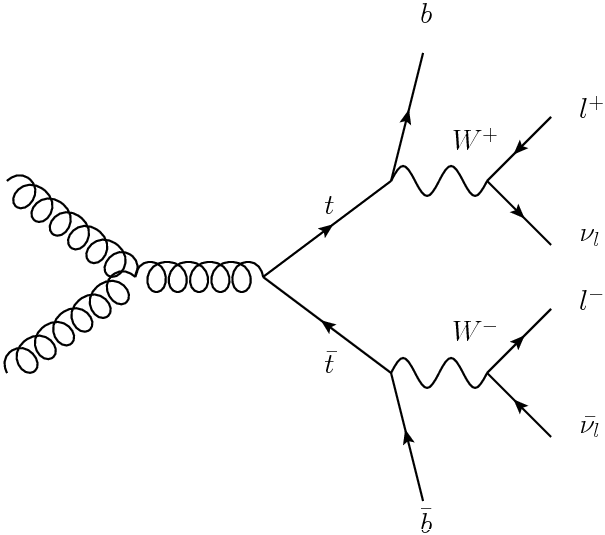
\includegraphics[width=0.4\textwidth]{figures/search_stop2l/strategy/fgraph_ttbar}
        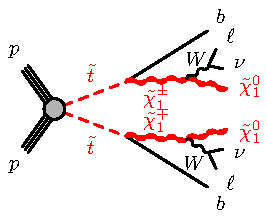
\includegraphics[width=0.4\textwidth]{figures/search_stop2l/strategy/fgraph_stop_bCN}
        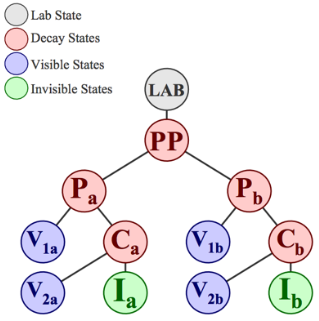
\includegraphics[width=0.5\textwidth]{figures/search_stop2l/strategy/RJRtree_generic_PPviaC}
        \caption{
            An example of an RJR decay tree interpretation of physics processes.
            The RJR decay tree (\textit{\textbf{bottom}}) can be fit to both the \ttbar~decay
            (\textit{\textbf{upper left}}) or the $\stopone \rightarrow b \chinoonepm$ process (\textit{\textbf{upper right}}).
            Each of the upper processes \textit{topologically} matches that of the RJR decay tree, but
            the underlying differences in their kinematics means that kinematic observables derived
            from this RJR decay tree may provide means of discrimination between the two.
            Each circle in the RJR decay tree represents a reconstructed reference frame,
            characterised by its own four-vector information.
        }
        \label{fig:rjr_ttbar_bcn}
    \end{center}
\end{figure}

\FloatBarrier
%%%%%%%%%%%%%%%%%%%%%%%%%%%%%%%%%%%%%%%%%%%%%%%%%%%%%%%%%%%%%%%%%%%%%%%%%%%
%%%%%%%%%%%%%%%%%%%%%%%%%%%%%%%%%%%%%%%%%%%%%%%%%%%%%%%%%%%%%%%%%%%%%%%%%%%
%%%%%%%%%%%%%%%%%%%%%%%%%%%%%%%%%%%%%%%%%%%%%%%%%%%%%%%%%%%%%%%%%%%%%%%%%%%
%
% RJR FOR THREE BODY
%
%%%%%%%%%%%%%%%%%%%%%%%%%%%%%%%%%%%%%%%%%%%%%%%%%%%%%%%%%%%%%%%%%%%%%%%%%%%
%%%%%%%%%%%%%%%%%%%%%%%%%%%%%%%%%%%%%%%%%%%%%%%%%%%%%%%%%%%%%%%%%%%%%%%%%%%
%%%%%%%%%%%%%%%%%%%%%%%%%%%%%%%%%%%%%%%%%%%%%%%%%%%%%%%%%%%%%%%%%%%%%%%%%%%

The RJR decay tree imposed in the present analysis searching for the three-body decay
of the \stopone quark is presented in Figure~\ref{fig:rjr_stop}.
The visible system ($V_a + V_b$) is provided only the two leptons in the event.
The invisible system ($I_a + I_b$) is provided the missing transverse momentum.

\begin{figure}[!htb]
    \begin{center}
        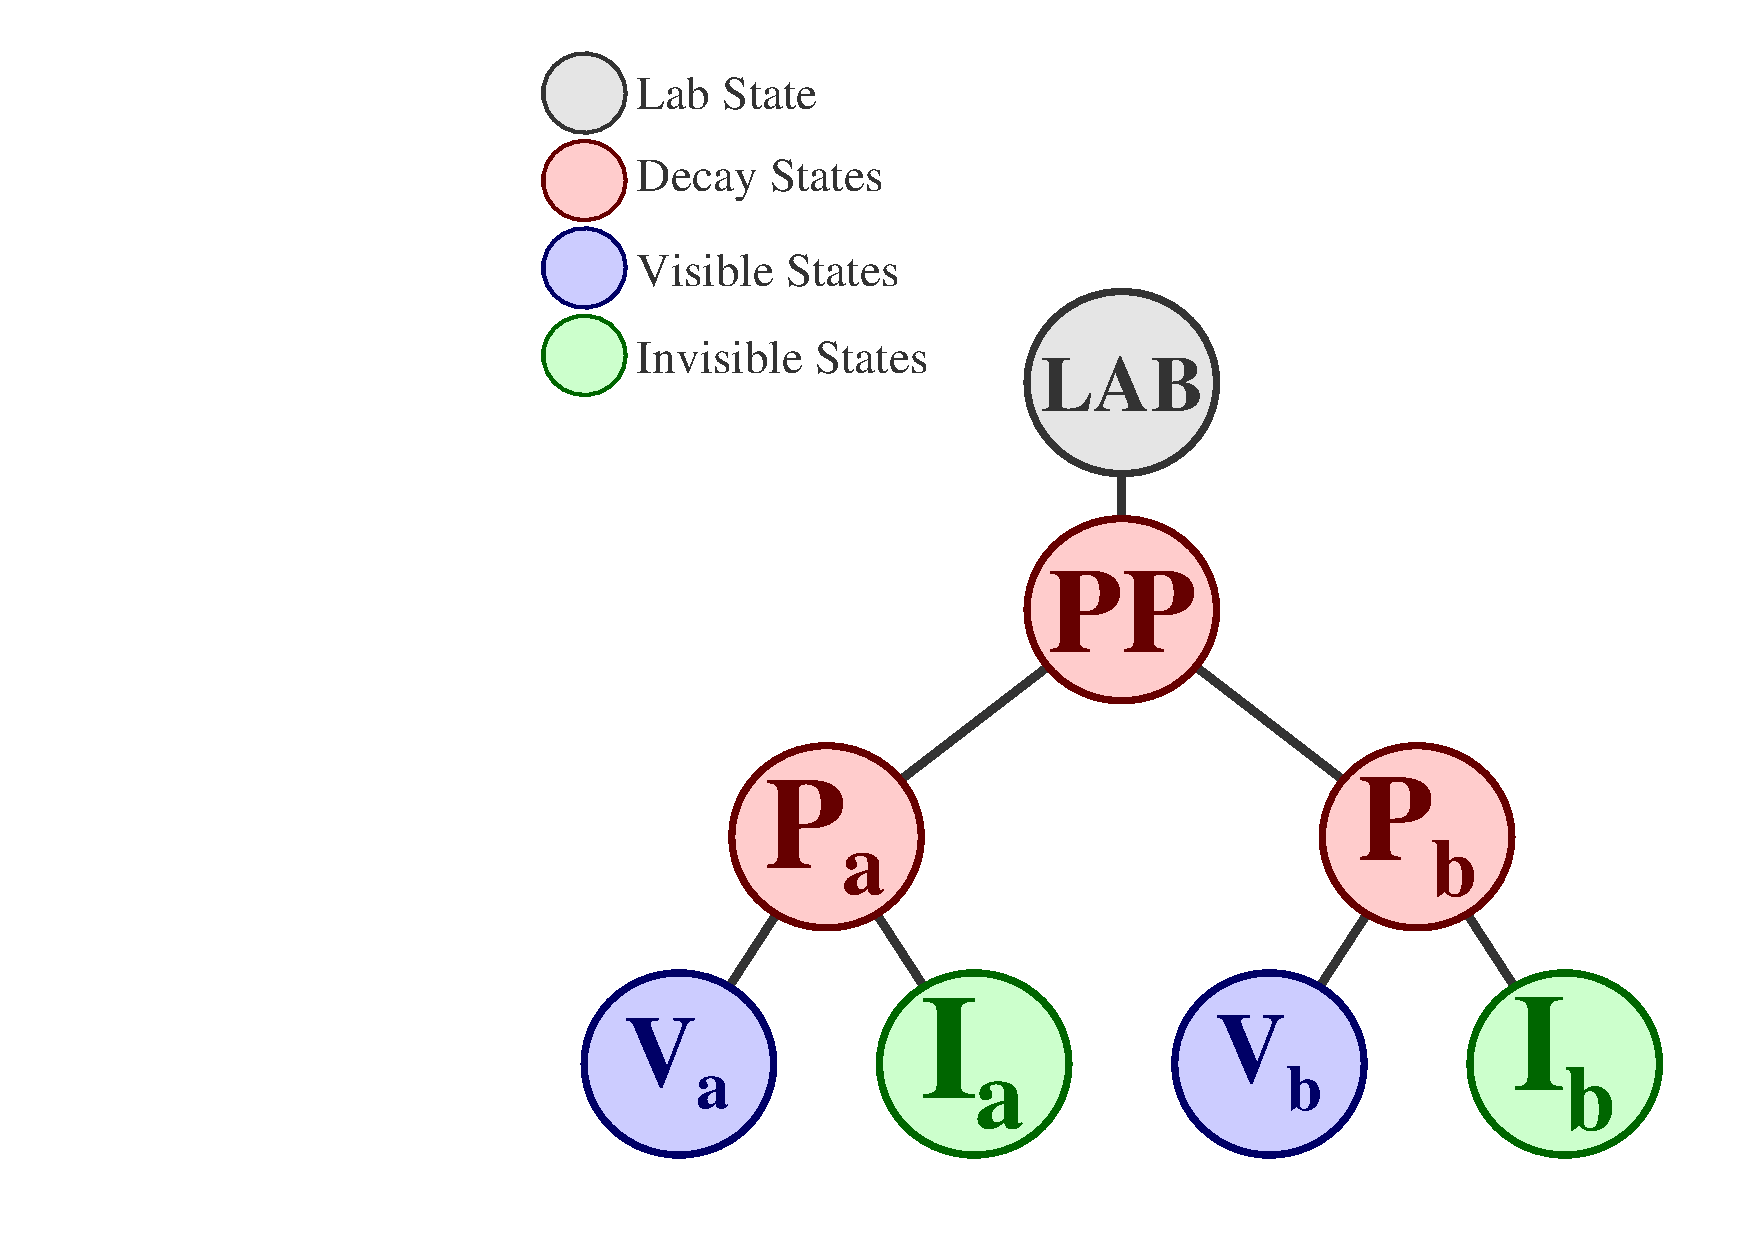
\includegraphics[width=0.6\textwidth]{figures/search_stop2l/strategy/RJRtree_DiSparticle}
        \caption{
            RJR decay tree assumption used in the 2015+2016 analysis searching for the
            three-body decay of the \stopone quark, $\stopone \rightarrow b W \ninoone$.
            It is the most general decay tree for $R$-parity conserving SUSY scenarios in
            which pair-produced sparticles ($P_a$ and $P_b$) each decay to visible states ($V_a$ and $V_b$)
            and invisible states ($I_a$ and $I_b$).
            Each of the final states ($V_i$ and/or $I_i$) may, in principle, be composed of multiple particles.
            In the present analysis, only the two leptons in the event are provided as inputs to the $V_i$ and both
            are required to be non-empty (i.e. $V_a$ is one of the leptons, $V_b$ the other).
            The missing transverse momentum in the event is decomposed via a set of Jigsaw Rules into the
            states $I_a$ and $I_b$.
        }
        \label{fig:rjr_stop}
    \end{center}
\end{figure}

The RJR decay tree in Figure~\ref{fig:rjr_stop} is the most general RJR decay tree one can make for
targetting $R$-parity conserving SUSY models.
This decay tree makes the least number of assumptions on the decay of the pair-produced sparticles and
their children (if any).
This is beneficial, as developing a search (whose a-priori intent is for discovery of new physics)
that is largely dependent on the model assumed for designing the analysis' selection criteria
greatly limits the applicability and scope of that search.
For example, one can imagine using the decay tree of Figure~\ref{fig:rjr_ttbar_bcn} also for the three-body
decays considered in the present search, $\stopone \rightarrow b W \ninoone$.
However, the decay tree in Figure~\ref{fig:rjr_ttbar_bcn} assumpes that there is enough information to
kinematically separate the $b$-tagged jets and leptons into the $V_{1(a,b)}$ and $V_{2(a,b)}$ states,
respectively, therefore requiring at least four visible objects to be reconstructed.
As discussed in Section~\ref{sec:stop_final_state}, this is not the case for the three-body decays
of the \stopone relevant for the present analysis and so Figure~\ref{fig:rjr_ttbar_bcn} is not well-suited
for this search.
What we want, in the end, is a means to separate from the background the presence of an $R$-parity conserving
SUSY signal while making as few assumptions as possible.

As mentioned, the goal of the RJR technique is to provide a full accounting of all of the states specified by the
user in the imposed RJR decay tree; or, at least a close and/or optimal approximation of them.
Unfortunately, it is in generall impossible to do this as a result of the presence of multiple weakly interacting
particles in the final state and, less generally, because of combinatoric ambiguities
that make it difficult to assign objects to specific locations in the decay (e.g. associating $b$-jets to
the correct side of the decay).
The RJR technique and its so-called Jigsaw Rules provide a means to systematically resolve these unknowns
on an event-by-event basis.

In order to resolve combinatoric ambiguities amongst the reconstructed visible objects so that they may
be grouped `correctly', one can employ a Jigsaw Rule for performing a recursive partitioning
of the visible objects until that grouping which minimizes the visible mass of each side of a decay vertex is found.
This is not necessarily the true grouping, but it is a method that is found to reproduce well, on average,
the correct grouping of objects.

In the RJR decay tree used in the search for $\stopone \rightarrow b W \ninoone$, illustrated
in Figure~\ref{fig:rjr_stop}, there are 6 under-constrained degrees-of-freedom (DOF) due to the
weakly interacting particles/missing transverse momentum.
These are (2 DOF for each) as follows:
\begin{itemize}
    \item The longitudinal momenta of the $I_i$ states: $p_{I_i,z}$
    \item The splitting of the missing transverse momentum between the $I_i$ states: $\bm{p}_{I_a,T} + \bm{p}_{I_b,T} = \bm{E}_T^{\text{miss}}$
    \item The mass of the di-invisible system composed of $I_a$ and $I_b$: $m_I$ ($m_{I_a}$ and $m_{I_b}$)
\end{itemize}
The RJR technique sets out to provide values for these unknowns through assumptions (constraints) that it makes
for determining the relative velocities (boosts) between rest-frames indicated by the circles in Figure~\ref{fig:rjr_stop}.
The recursive element of the technique is most obvious in this respect: the algorithm moves from
the first known reference frame (the lab frame) and traverses down the decay tree using information
only from the current frame to determine the boosts for moving into the next reference frame.
That is, with respect to Figure~\ref{fig:rjr_stop}, information only from the lab frame
is used to move to the $PP$ (center-of-mass, COM) frame and information from this COM frame
is used to move to either of the respective $P_i$ frames.
There are specific Jigsaw Rules at each step of this navigating of the RJR decay tree that determine
\textit{how} the information in each of these frames is used simultaneously to move to the next
and to provide estimates of the under-constrained DOF mentioned above.

The first step that the RJR technique takes in constructing the boosts relating the reference frames is to
determine the mass of the invisible system, $m_I$, composed of the states $I_a$ and $I_b$.
This information is required to be able to consistently perform boosts between the reference frames while
keeping each side, or \textit{hemisphere}, of the decay balanced against the other.
This means that, generally, the di-invisible system will have non-trivial opening angles between the $I_i$
states in order to balance the visible system frame-by-frame.
This means that it will attain a mass\footnote{From special relativistic mechanics, the mass of a system comprised
of two subsystems, 1 and 2, is generally given by $m_{12}^2 = m_1^2 + m_2^2 + 2(E_1E_2 - |\vec{p}_1| |\vec{p}_2| \cos \theta_{12})$,
where $\theta_{12}$ is the opening angle between $\vec{p}_1$ and $\vec{p}_2$.}
To satisfy this balancing requirement, the RJR technique takes for $m_I$ the smallest Lorentz-invariant
mass consistent with the input lab-frame observables that will accomodate the subsequent boosts and also prevent
the states $I_i$ from becoming tachyonic.
For the decay tree in Figure~\ref{fig:rjr_stop} this turns out to be,
\begin{align}
    m_I^2 = m_V^2 - 4m_{V_a} m_{V_b},
    \label{eq:rjr_invisible_mass}
\end{align}
where $V$ refers to the total visible system comprised of $V_a$ and $V_b$.

Next, the RJR technique determines the boost from the lab to the $PP$ (COM) frame.
To determine this boost, we must determine the longitudinal momentum of the invisible system, $p_{I,z}^{\text{Lab}}$,
which is one of the under-constrained DOF.
The RJR technique chooses this value such that the rapidity of the visible and invisible systems are equal.
This choice results in our choice of the $PP$ (COM) reference frame being a longitudinally boost-invariant
choice, meaning that all subsequent observables derived in the RJR decay tree will also be
longitudinally boost-invariant.
Additionally, one can see that this also forces the mass of the $PP$ system, $m_{V+I}$, to
take its minimum value.\footnote{This is een using the previous footnote and knowledge that $\vec{E}_T^{\text{miss}}$
must balance the visible system's transverse momentum.}

With the longitudinal momentum of the invisible system determined, along with its mass, we have
the expression for the boost relating the lab frame to the $PP$ (COM) frame:
\begin{align}
    \vec{\beta}_{PP}^{\,\text{LAB}} = \frac{
        \vec{p}_{PP}^{\text{LAB}}
    }
    {
        E_{PP}^{\text{LAB}}
    }
    = \frac{
        \vec{p}_V^{\,\text{LAB}} + \vec{p}_I^{\,\text{LAB}}
    }
    {
        E_V^{\text{LAB}} + \sqrt{ |\vec{p}_I^{\,\text{LAB}} |^2 + m_I^2 }
    }.
    \label{eq:rjr_lab_boost}
\end{align}
The boost in Equation~\ref{eq:rjr_lab_boost} affords provides us the observables in the $PP$ (COM)
reference frame.
We must use information in this frame to determine how to move to the individual sparticle frames, $P_i$.
This will provide us with the last set of information regarding how the missing transverse momentum
is to be shared between the states $I_i$.
Here, the RJR technique makes the assumption that $m_{V_a} = m_{V_b}$, which, in the context of the processes
considered, is reasonable.
As we are in the COM frame, this choice for the masses of the $V_i$ states dictates that the boosts of each of their
individual reference frames be equal in magnitude and anti-parallel.
For our decay tree, a possible solution for this is chosen to be:
\begin{align}
    \vec{\beta}_{P_i}^{\,PP} = \frac{
        \vec{p}_{V_a}^{\,PP} - \vec{p}_{V_b}^{\,PP}
    }
    {
        E_{V_a}^{PP} + E_{V_b}^{PP}
    }.
    \label{eq:rjr_pi_boost}
\end{align}
Under this boost, all observables subsequently defined are \textit{contra-boost invariant}, meaning that,
as in the case for the longitudinal boost invariance described previously, all observables
are therefore insensitive (on average) to the fact that this boost from the $PP$ (COM) frame to the $P_i$
frames is not necessarily the true boost.
Indeed, this final contra-boost invariance is the main motivation behind the structure of Equation~\ref{eq:rjr_pi_boost}.

Now that we have the boost $\vec{\beta}_{P_i}^{\,PP}$ to the $P_i$ frames, one can determine the splitting of invisible
momentum by requiring $\vec{p}_{V_i}^{\,P_i} + \vec{p}_{I_i}^{\,P_i} = 0$, which
is the final under-constrained DOF of the RJR decay tree relevant to the analysis being presented.

With the application of the RJR technique, then, all of the unknowns in the event are thus determined
(approximately), and one has access to kinematic information (four vectors) for every level of the RJR decay tree
that has been imposed (Figure~\ref{fig:rjr_stop}).

\FloatBarrier
%%%%%%%%%%%%%%%%%%%%%%%%%%%%%%%%%%%%%%%%%%%%%%%%%%%%%%%%%%%%%%%%%%%%%%%%%%%
%%%%%%%%%%%%%%%%%%%%%%%%%%%%%%%%%%%%%%%%%%%%%%%%%%%%%%%%%%%%%%%%%%%%%%%%%%%
%%%%%%%%%%%%%%%%%%%%%%%%%%%%%%%%%%%%%%%%%%%%%%%%%%%%%%%%%%%%%%%%%%%%%%%%%%%
%
% DISCRIMINATING VARIABLES
%
%%%%%%%%%%%%%%%%%%%%%%%%%%%%%%%%%%%%%%%%%%%%%%%%%%%%%%%%%%%%%%%%%%%%%%%%%%%
%%%%%%%%%%%%%%%%%%%%%%%%%%%%%%%%%%%%%%%%%%%%%%%%%%%%%%%%%%%%%%%%%%%%%%%%%%%
%%%%%%%%%%%%%%%%%%%%%%%%%%%%%%%%%%%%%%%%%%%%%%%%%%%%%%%%%%%%%%%%%%%%%%%%%%%

\subsection{Discriminating Observables}
\label{sec:stop_variables}

In this section we describe the basis of kinematic observables, defined using the states defined
by the RJR, that are used to define the SRs, CRs, and VRs in the present analysis.

With the RJR technique providing us with an approximation of the center-of-mass frame of the
\stop system (the state $PP$ in Figure~\ref{fig:rjr_stop}), a natural variable to define is the
total energy, or invariant mass, available to those objects in our decay tree.
With the entire system defined, this can be obtained easily and we refer to this
appriximate COM energy as $m_{PP}$, shown in Figure~\ref{fig:rjr_mpp}.

\begin{figure}[!htb]
    \begin{center}
        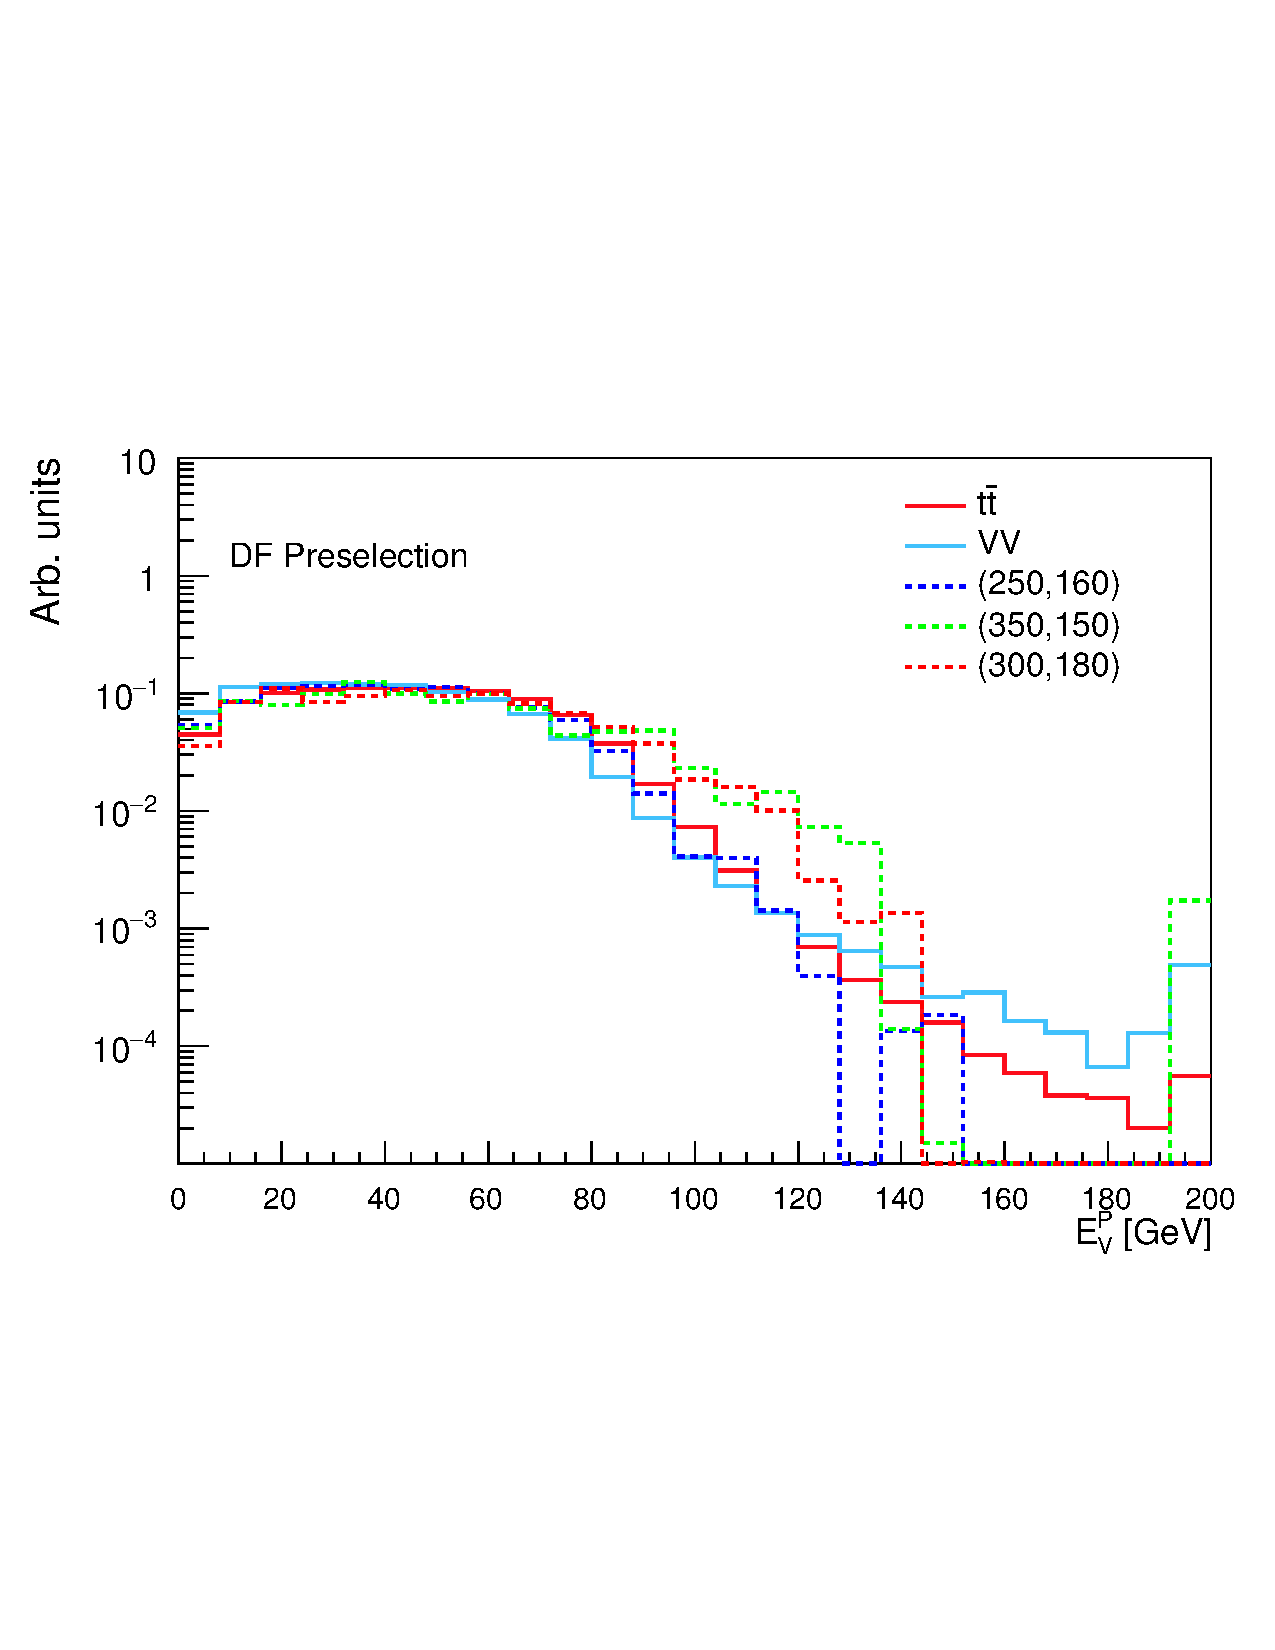
\includegraphics[width=0.7\textwidth]{figures/search_stop2l/strategy/comp_plots/dfpresel_MDR}
        \caption{
            Normalised distribution of the $m_{PP}$ variable for several $\stopone \rightarrow b W \ninoone$
            signal hypotheses, labeled with respect to their assumed $(m_{\stopone}, m_{\ninoone})$ values in the
            legend.
            The SM \ttbar~and diboson ($VV$) background processes are also shown for comparison.
        }
        \label{fig:rjr_mpp}
    \end{center}
\end{figure}

In addition to $m_{PP}$, we can define the associated transverse momentum of the COM frame,
$|\vec{p}_T^{\,PP}|$, shown in Figure~\ref{fig:rjr_pTT_T}.
Used in conjunction, the two variables $m_{PP}$ and $|\vec{p}_T^{\,PP}|$ can be used to build the
ratio, $R_{p_T}$, defined as:
\begin{align}
    R_{p_T}  = \frac{
        |\vec{p}_T^{\,PP}|
    }
    {
        |\vec{p}_T^{\,PP}| + m_{PP}/4
    }.
    \label{eq:rjr_rpt}
\end{align}
Distributions of $R_{p_T}$ are provided in Figure~\ref{fig:rjr_RPT}.
The more central nature of our signal hypothesis wherein the pair-produced sparticles decay to
heavy final state objects and distribute more of their energy to the transverse plane can be seen
in Figure~\ref{fig:rjr_RPT}.

\begin{figure}[!htb]
    \begin{center}
        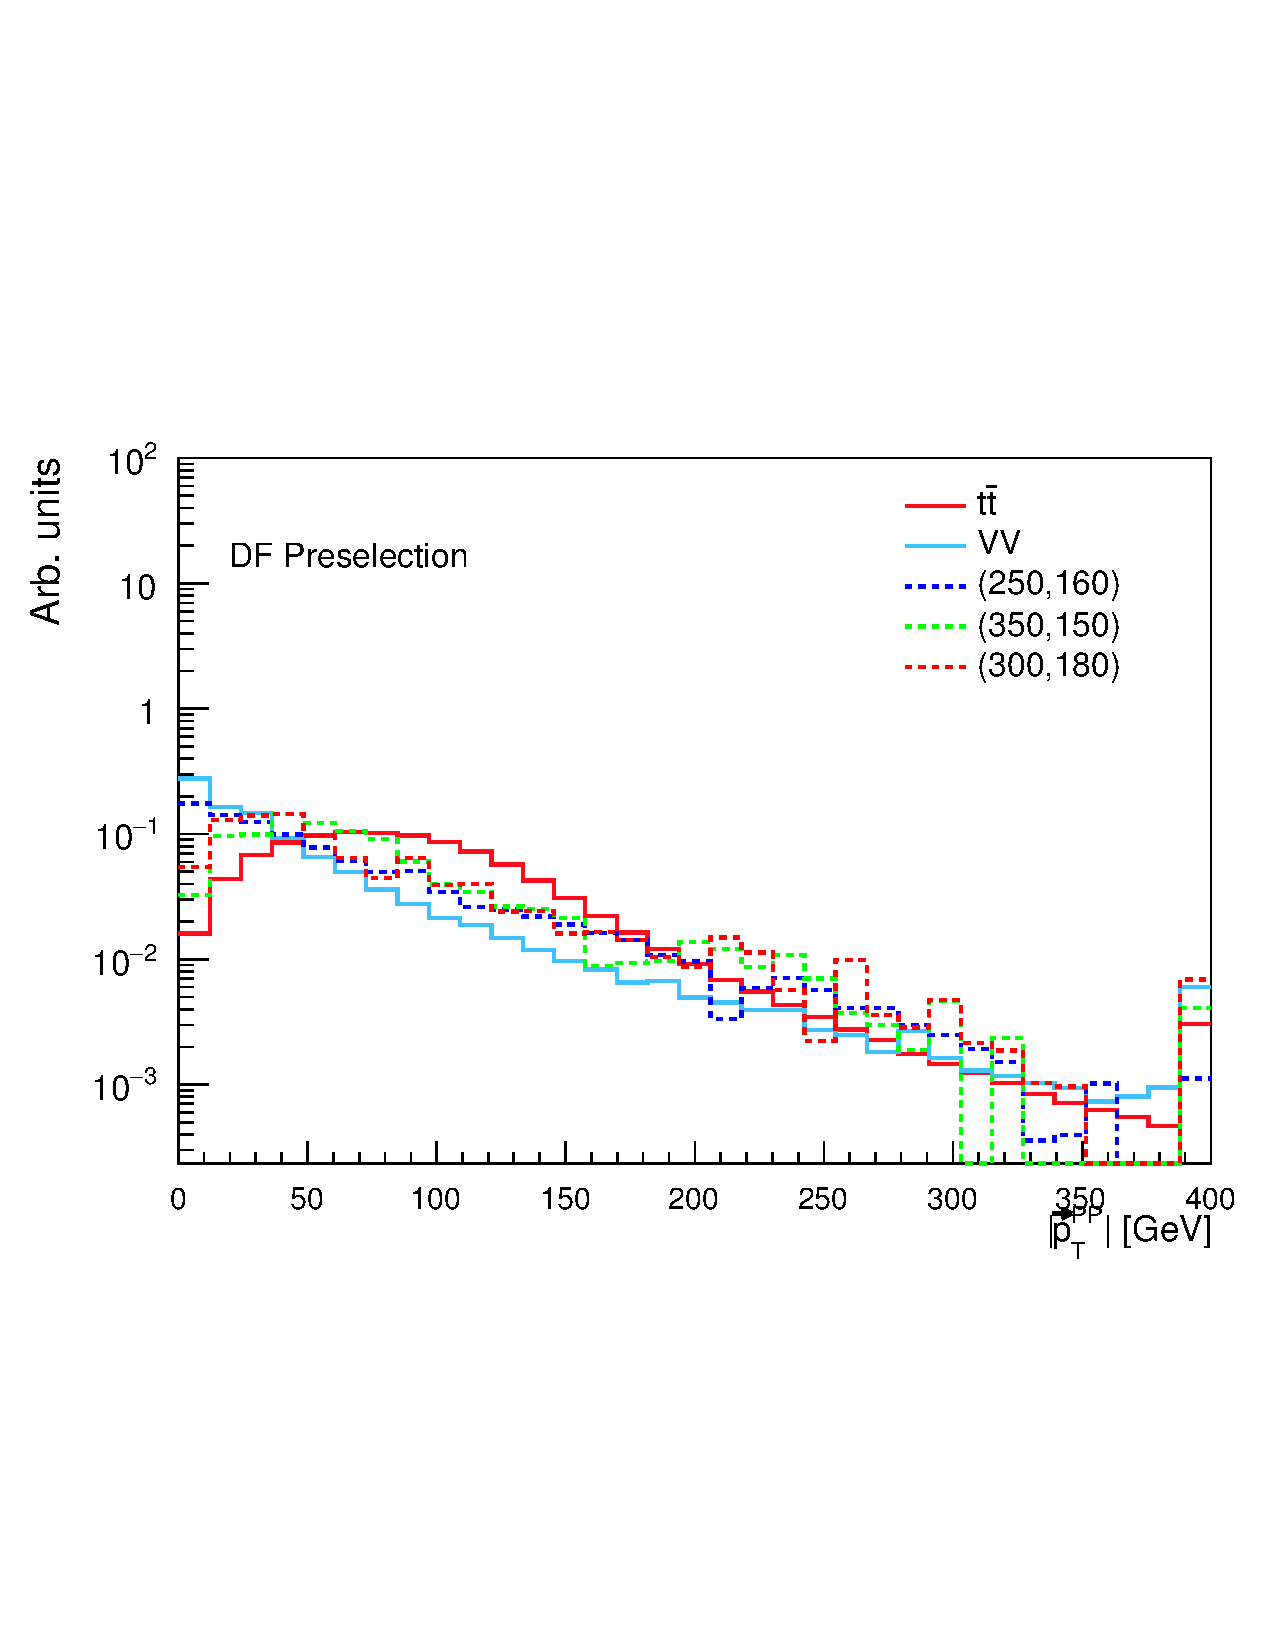
\includegraphics[width=0.7\textwidth]{figures/search_stop2l/strategy/comp_plots/dfpresel_pTT_T}
        \caption{
            Normalised distribution of the $|\vec{p}_T^{\,PP}|$ variable for several $\stopone \rightarrow b W \ninoone$
            signal hypotheses, labeled with respect to their assumed $(m_{\stopone}, m_{\ninoone})$ values in the
            legend.
            The SM \ttbar~and diboson ($VV$) background processes are also shown for comparison.
        }
        \label{fig:rjr_pTT_T}
    \end{center}
\end{figure}

\begin{figure}[!htb]
    \begin{center}
        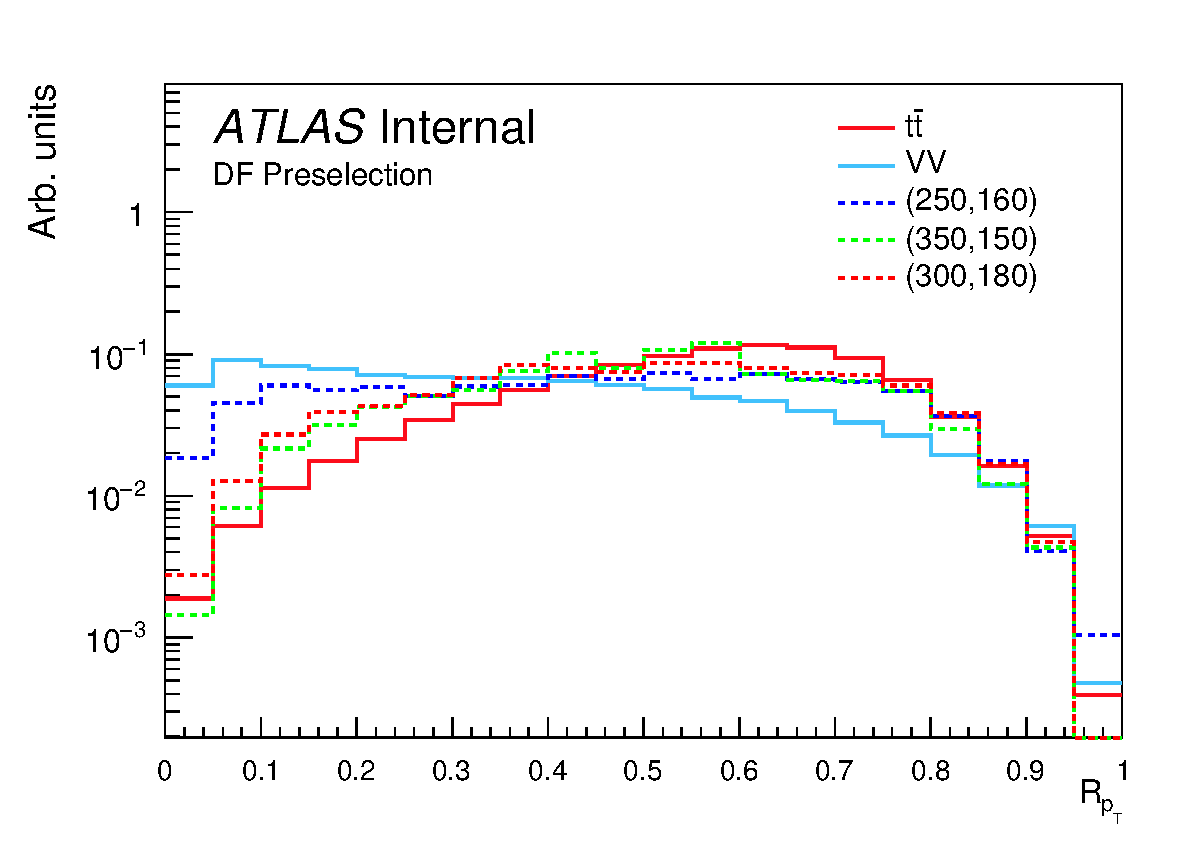
\includegraphics[width=0.7\textwidth]{figures/search_stop2l/strategy/comp_plots/dfpresel_RPT}
        \caption{
            Normalised distribution of the $R_{p_T}$ variable for several $\stopone \rightarrow b W \ninoone$
            signal hypotheses, labeled with respect to their assumed $(m_{\stopone}, m_{\ninoone})$ values in the
            legend.
            The SM \ttbar~and diboson ($VV$) background processes are also shown for comparison.
        }
        \label{fig:rjr_RPT}
    \end{center}
\end{figure}

The next variable that can be defined uses the relative velocity of the $PP$ frame as seen
in the LAB frame, as well as the total visible system $V = V_a + V_b$ as seen in the $PP$ frame.
This is the azimuthal angle between the velocity, or boost, from the LAB to $PP$ frame and the visible
system $V$ (which, in our case, is simply the dilepton system) as seen in the $PP$ (COM) frame.
This variable, \dpb, is shown in Figure~\ref{fig:rjr_DPB}.

The key features of the angular quantity \dpb can be seen in Figure~\ref{fig:rjr_DPB}.
The \stopone signals cleary peak more strongly near values of $\dpb \sim \pi$ and are roughly
overlapping for all values of $\sdiff$, meaning that the behavior of \dpb is loosely
independent on \sdiff.
Rather, \dpb tends to be more dependent on the assumptions gone into constructing the underlying
RJR decay tree in Figure~\ref{fig:rjr_stop}, from which the quantity \dpb is ultimately derived.
As discussed, with the dilepton system $V = V_a + V_b$, Equation~\ref{eq:rjr_invisible_mass} results
in the assumption $m_I = m_V$.
For the massive \ninoone particles in the invisible final state of our \stopone signal decays, this
assumption is clearly incorrect and means that the boost from the LAB frame to the approximate 
$PP$ (COM) frame tends to be an \textit{over}-boost since the assumption of equal masses assumes
too much momentum for the invisible system.
In reality, on the other hand, much of the \stopone energy-momentum goes
into the \textit{mass} of the invisible system.
This over-boosting can be seen in Equation~\ref{eq:rjr_lab_boost} with the under-predicted $m_I$
in the denominator.
This results in the system $V$ to point, on average, in the opposite (anti-parallel) direction with
respect to the boost in Equation~\ref{eq:rjr_lab_boost} when viewed in the approximate COM frame, $PP$.

\begin{figure}[!htb]
    \begin{center}
        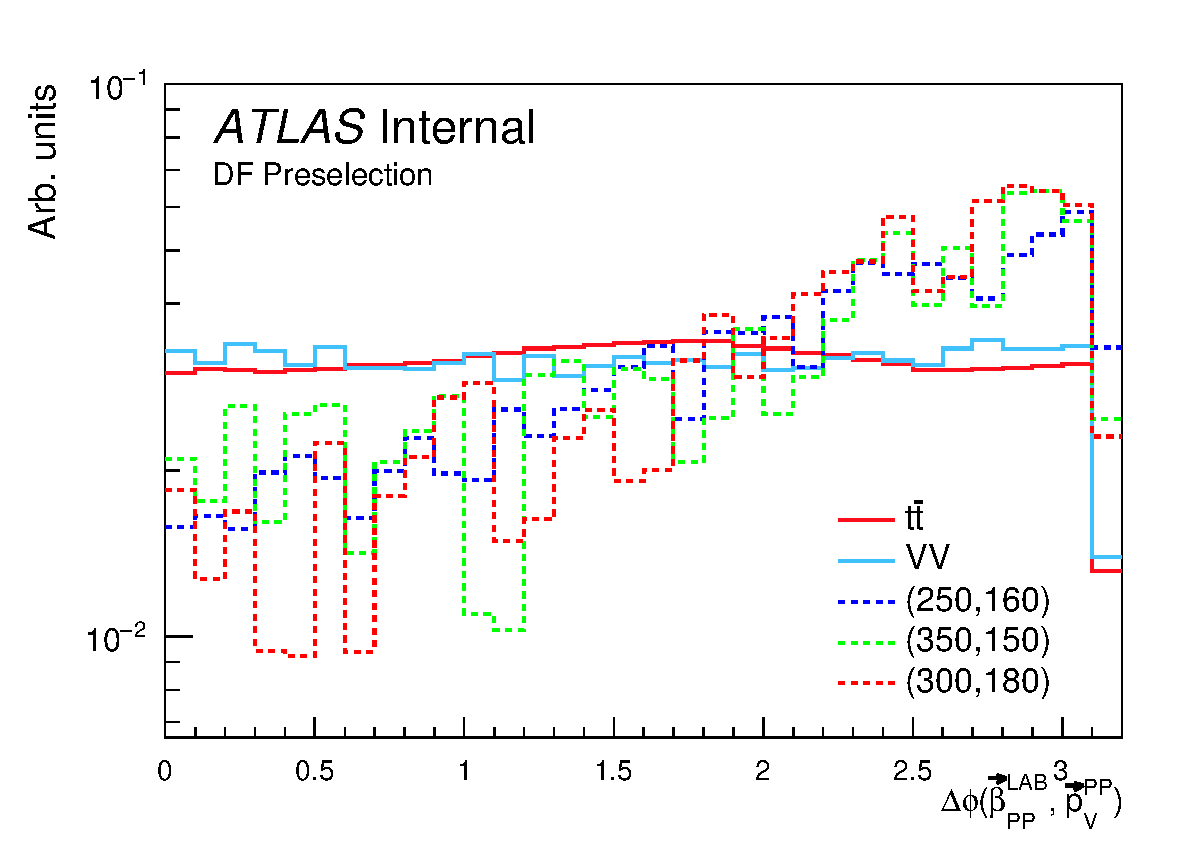
\includegraphics[width=0.7\textwidth]{figures/search_stop2l/strategy/comp_plots/dfpresel_DPB_vSS}
        \caption{
            Normalised distribution of the $\dpb$ variable for several $\stopone \rightarrow b W \ninoone$
            signal hypotheses, labeled with respect to their assumed $(m_{\stopone}, m_{\ninoone})$ values in the
            legend.
            The SM \ttbar~and diboson ($VV$) background processes are also shown for comparison.
        }
        \label{fig:rjr_DPB}
    \end{center}
\end{figure}

We can also define a variable that is sensitive to the (squared) mass differences between the pair-produced
\stopone and final state \ninoone.
This observable, corresponding to the energy of one of the $V_i$ (one of the leptons) with respect to the sparticle $P_i$ frames
of reference.
This variable, $E_V^P$, can be interpreted as the approximate energy of the state $V_i$ in the frame
corresponding to $P_i$ and has an endpoint following,
\begin{align}
    E_V^P \propto \frac{
        m_{P_i}^2 - m_{I_i}^2
    }
    {
        m_{P_i}
    },
    \label{eq:mdr_endpoint}
\end{align}
which follows essentially from special relativistic kinematics.
Distributions of $E_V^P$ are given in Figure~\ref{fig:rjr_MDR}.

\begin{figure}[!htb]
    \begin{center}
        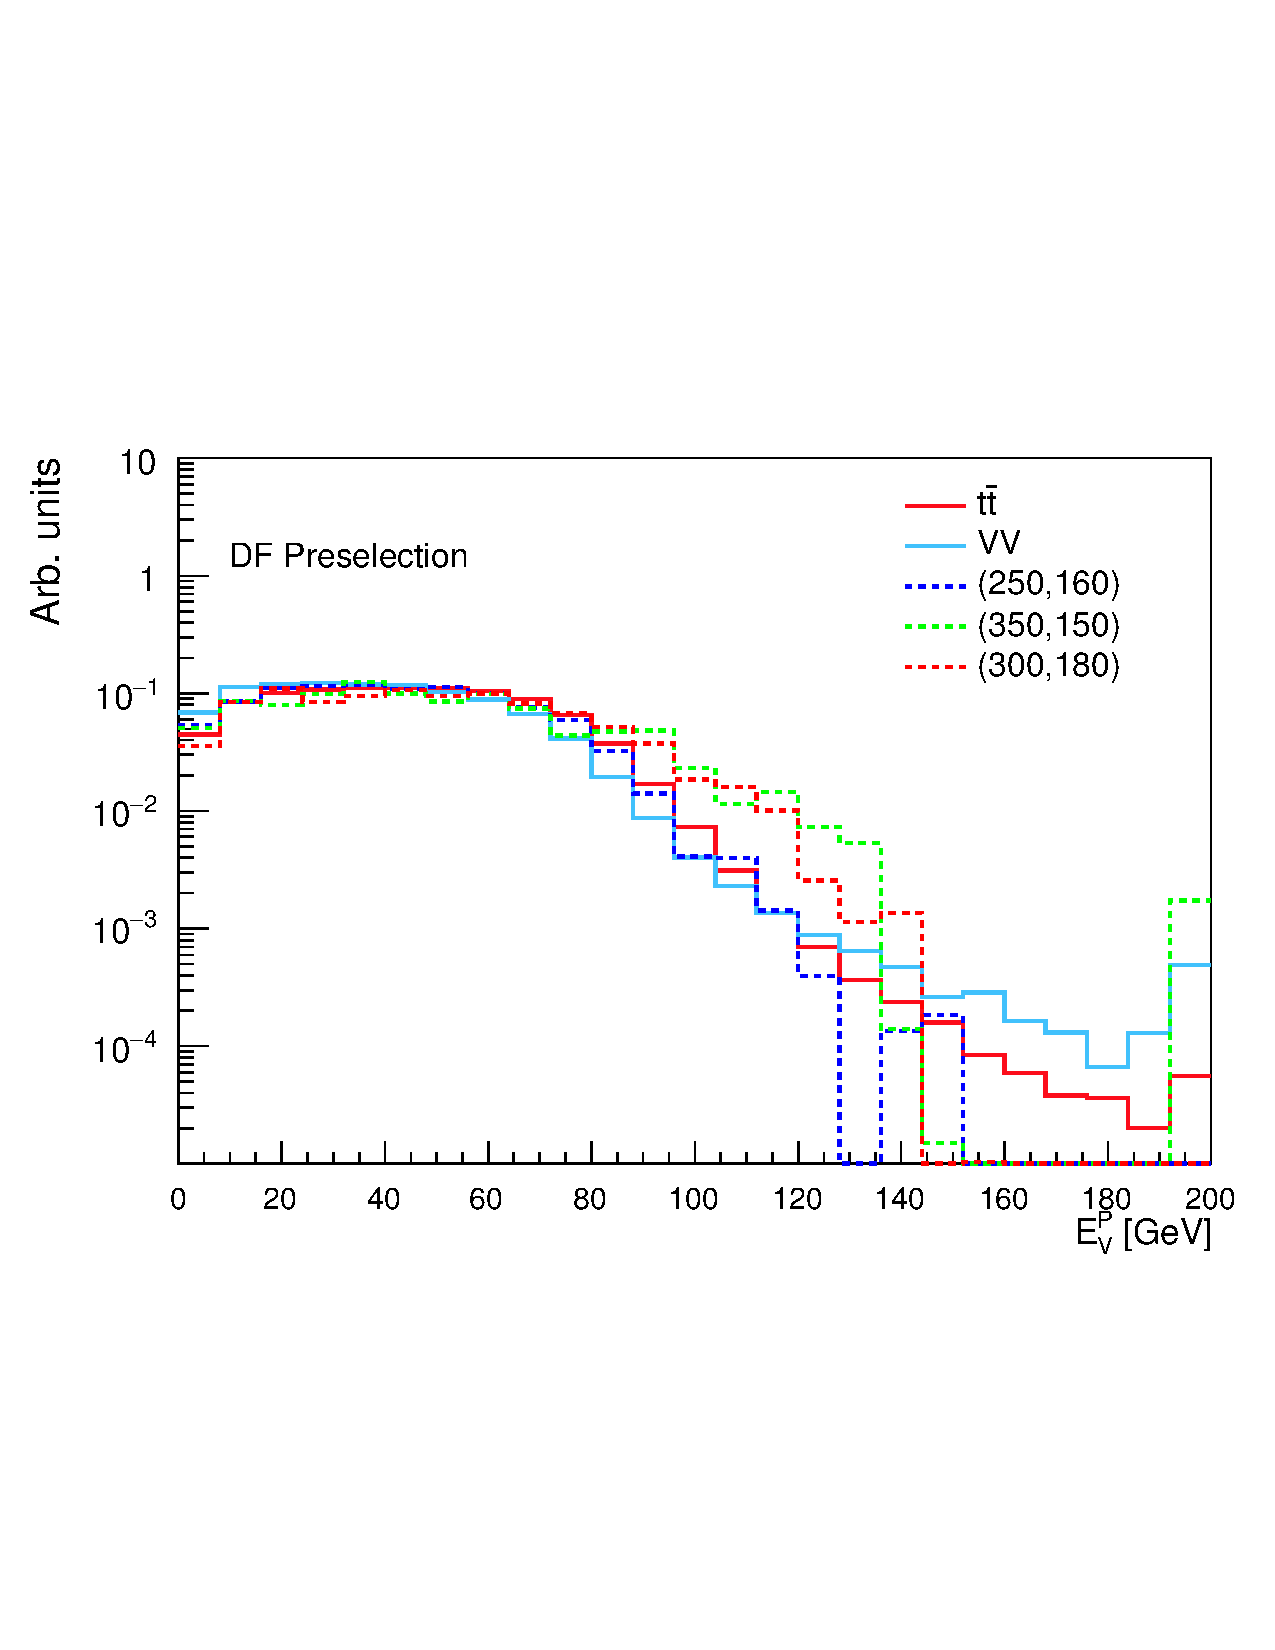
\includegraphics[width=0.7\textwidth]{figures/search_stop2l/strategy/comp_plots/dfpresel_MDR}
        \caption{
            Normalised distribution of the $\mdr$ variable for several $\stopone \rightarrow b W \ninoone$
            signal hypotheses, labeled with respect to their assumed $(m_{\stopone}, m_{\ninoone})$ values in the
            legend.
            The SM \ttbar~and diboson ($VV$) background processes are also shown for comparison.
        }
        \label{fig:rjr_MDR}
    \end{center}
\end{figure}

The next Jigsaw variable to be used is the so-called `visible shape' of the $PP$ (COM) frame.
In the limiting case of $m_{V_a} = m_{V_b} = 0$, in which the current analysis finds itself,
this quantity corresponds to the (inverse) boost factor ($\gamma$) associated with the boost from the
$PP$ frame to the $P_i$ frames and is defined as follows,
\begin{align}
    \text{PP Visible Shape} \rightarrow \gaminv \equiv \frac{
        \sqrt{
            2(|\vec{p}_{V_a}^{\,PP}| |\vec{p}_{V_b}^{\,PP}| + \vec{p}_{V_a}^{\,PP} \cdot \vec{p}_{V_b}^{\,PP})
        }
    }
    {
        |\vec{p}_{V_a}^{\,PP}| + |\vec{p}_{V_b}^{\,PP}|.
    }.
    \label{eq:rjr_gaminv}
\end{align}
The quantity \gaminv is a measure of how the two visible systems, $V_i$, are distributed.
It tends towards unity when $V_a$ and $V_b$ (the two leptons) are equal in momenta and collinear while tending
towards zero when they are back-to-back or having different momenta.
In this sense, the variable earns its name as a measure of the `visible shape' of the decay.
In decays with massive particles contributing to the missing tansverse momentum,
the visible final state legs $V_a$ and $V_b$ will, on average, tend to not be back-to-back since,
in addition to balancing each other, they much balance the invisible particles.
This effect is exaggerated in two cases: (1) when the decay is highly `active' (as in \ttbar),
and (2) when the invisible system is composed of heavy particles.
The effect (1) is essentially due to our including in the states $V_a$ and $V_b$ only the
final state leptons: the quantity \gaminv is blind to any jets in the event and the `shape' it
corresponds to is in response to balancing these jets as well.
The effect (2) results in the visible legs recoiling harder off of the heavier invisible particles,
thus tending to be collinear.
Distributions of the \gaminv quantity are shown in Figure~\ref{fig:rjr_gaminv}.

\begin{figure}[!htb]
    \begin{center}
        \includegraphics[width=0.7\textwidth]{figures/search_stop2l/strategy/comp_plots/dfpresel_gamInvRP1}
        \caption{
            Normalised distribution of the $\gaminv$ variable for several $\stopone \rightarrow b W \ninoone$
            signal hypotheses, labeled with respect to their assumed $(m_{\stopone}, m_{\ninoone})$ values in the
            legend.
            The SM \ttbar~and diboson ($VV$) background processes are also shown for comparison.
        }
        \label{fig:rjr_gaminv}
    \end{center}
\end{figure}

The variables discussed so far are relatively independent of the underlying signal model
that we are attempting to search for.
Their utility relies simply on their being massivle particles contributing to the missing
transverse momentum.

We now discuss a variable that, in order for it to be useful in the search for \stopone particles,
makes an assumption on the nature of the pair-produced sparticle that we are
searching for.
This variable, \cosb, is angular in nature that is sensitive to the decay angle of a given lepton with
respect to the beam axis in it's production frame.

We define \cosb using only the two final state leptons.
Each of the leptons is boosted into the frame of the dilepton system, after which
we take the difference in pseudorapidities of the leptons in this frame,
$\Delta \eta_{\ell \ell} = \eta^+ - \eta^-$, where $\eta^+$ ($\eta^-$) refers to the
pseudorapidity of the positively (negatively) charged lepton.
The quantity \cosb is then defined as,
\begin{align}
    \cosb = \tanh ( \Delta \eta_{\ell\ell} / 2),
    \label{eq:rjr_cosb}
\end{align}
and is discussed further in Ref.~\cite{Melia:2011cu}.
As \cosb is sensitive to the projection angle of the lepton from its parent \stopone, it is
sensitive to the spin of the \stopone.
This can be seen in Figure~\ref{fig:rjr_cosb}, where we see that for the decay of the
spin-zero \stopone, the angular distribution is flatter and peaks at 0.
For the SM \ttbar~and $WW$ backgrounds, however, \cosb tends to peak at values $\pm 1$.

\begin{figure}[!htb]
    \begin{center}
        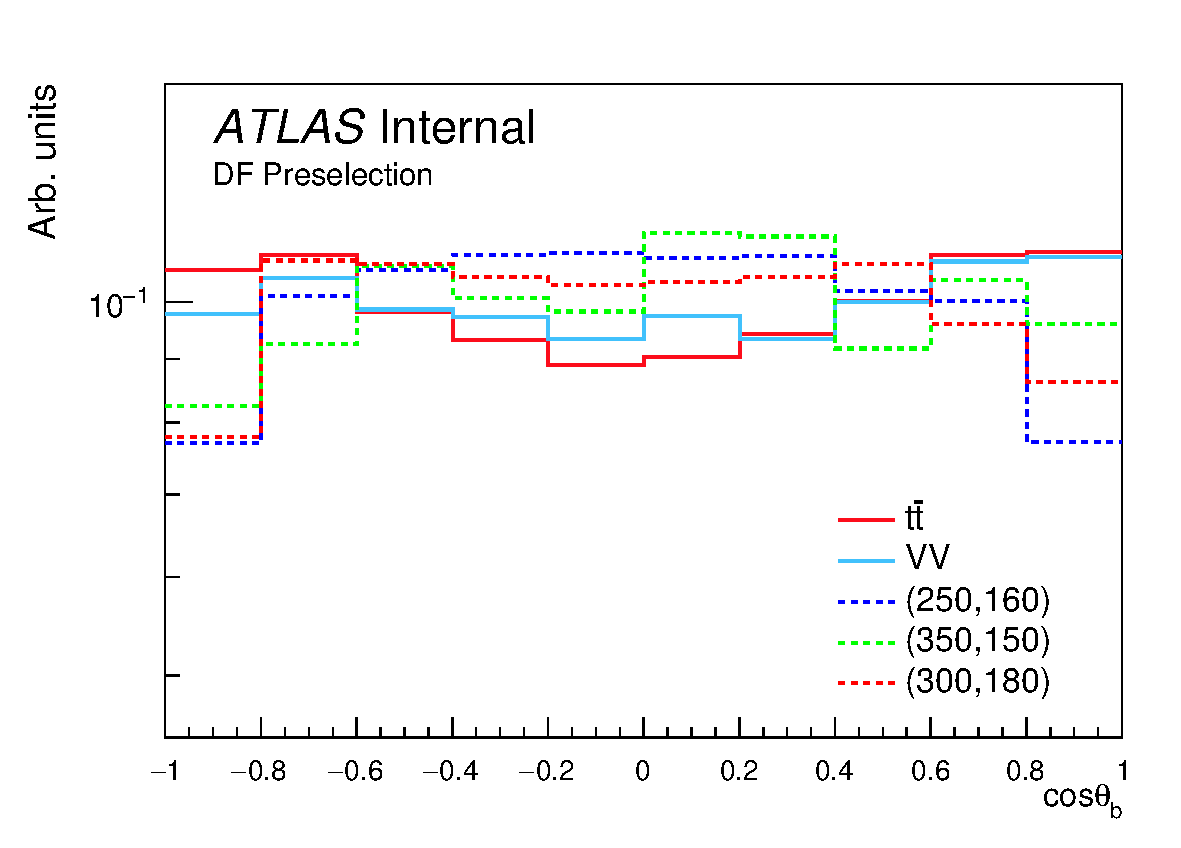
\includegraphics[width=0.7\textwidth]{figures/search_stop2l/strategy/comp_plots/dfpresel_cosThetaB}
        \caption{
            Normalised distribution of the $\cosb$ variable for several $\stopone \rightarrow b W \ninoone$
            signal hypotheses, labeled with respect to their assumed $(m_{\stopone}, m_{\ninoone})$ values in the
            legend.
            The SM \ttbar~and diboson ($VV$) background processes are also shown for comparison.
        }
        \label{fig:rjr_cosb}
    \end{center}
\end{figure}

In addition to the potential separation power between the decays of scalar \stopone particles
and the dominant SM backgrounds that \cosb exhibits in Figure~\ref{fig:rjr_cosb}, it should also
be noted that it is a longitudinally boost-invariant quantity.
It depends only on the \textit{difference} in pseudorapidities of the leptons, $\Delta \eta_{\ell\ell}$,
and thus is insensitive to our ignorance of the overall $z$-momenta in the event.
In this sense, the quantity \cosb follows very nicely the variables obtained from the RJR decay tree,
which are also motivated by longitudinal (and contra-) boost invariance.

\FloatBarrier
%%%%%%%%%%%%%%%%%%%%%%%%%%%%%%%%%%%%%%%%%%%%%%%%%%%%%%%%%%%%%%%%%%%%%%%%%%%
%%%%%%%%%%%%%%%%%%%%%%%%%%%%%%%%%%%%%%%%%%%%%%%%%%%%%%%%%%%%%%%%%%%%%%%%%%%
%%%%%%%%%%%%%%%%%%%%%%%%%%%%%%%%%%%%%%%%%%%%%%%%%%%%%%%%%%%%%%%%%%%%%%%%%%%
%
% SR DEF
%
%%%%%%%%%%%%%%%%%%%%%%%%%%%%%%%%%%%%%%%%%%%%%%%%%%%%%%%%%%%%%%%%%%%%%%%%%%%
%%%%%%%%%%%%%%%%%%%%%%%%%%%%%%%%%%%%%%%%%%%%%%%%%%%%%%%%%%%%%%%%%%%%%%%%%%%
%%%%%%%%%%%%%%%%%%%%%%%%%%%%%%%%%%%%%%%%%%%%%%%%%%%%%%%%%%%%%%%%%%%%%%%%%%%
\subsection{Signal Region Definitions}
\label{sec:stop_signal_region}

The definition of the SRs in the search for the three-body decay of the \stopone revolve around
two observations:
\begin{enumerate}
    \item The $\stopone \rightarrow b W \ninoone$ kinematics change rapidly as one traverses from
        the region near $\sdiff~ = ~m_{\text{top}}$ to that of $\sdiff~ = ~m_W$,
        as illustrated in Figure~\ref{fig:stop_phase_space}
    \item The angular quantities \cosb and \dpb,  sensitive to the presence of the scalar \stopone and massive
        \ninoone, respectively, allow for tight separation between the \stopone signal and dominant
        SM background processes
\end{enumerate}
The first item will ultimately result in the definition of two orthogonal SRs, one generally
more sensitive to the $\bWN$ decays nearer to the $\sdiff = m_{\text{top}}$ boundary
and the other being sensitive to those nearer to the $\sdiff = m_W$ boundary.
The primary method for defining SRs targetting these differing regimes is motivated by Figure~\ref{fig:stop_nbjets},
which shows that the \bWN decays with $\sdiff$ nearer to $m_W$, the reconstructed $b$-tagged
jet multiplicity tends to 0.
For this reason, the SRs targetting the $\sdiff \rightarrow m_W$ will require that the
candidate events have zero $b$-tagged jets, i.e. they apply a $b$-tagged jet \textit{veto} (`$b$-veto').
The SRs targetting the $\sdiff \rightarrow m_{\text{top}}$, on the other hand, will
require that there be at least one $b$-tagged jet in the candidate events.

The second item listed above is best illustrated by the distribution in Figure~\ref{fig:stop_corr2d_bveto}.
These two-dimensional distributions illustrate that the \bWN signal tends to populate
a different region in the two-dimensional space defined by $(\cosb, \dpb)$ than
the dominant dilepton SM backgrounds composed of \ttbar~and diboson production.
For this reason, the SRs will be further characterised by applying a selection within
the two-dimensional basis defined by the \cosb and \dpb variables.
Figure~\ref{fig:stop_corr2d_b} shows similar distributions as those presented in Figure~\ref{fig:stop_corr2d_bveto},
but illustrates that the relationship observed in the latter persist after
requiring that there be $b$-tagged jets in the events (the former distributions require a $b$-veto).
The fact that the $(\cosb, \dpb)$ relationship holds roughly independent of the $b$-tagged
jet multiplicity means that the same selection in this two-dimensional plane
can be applied for the SRs targetting both \bWN regimes, $\sdiff \rightarrow m_W$ and
$\sdiff \rightarrow m_{\text{top}}$.


\begin{figure}[!htb]
    \begin{center}
        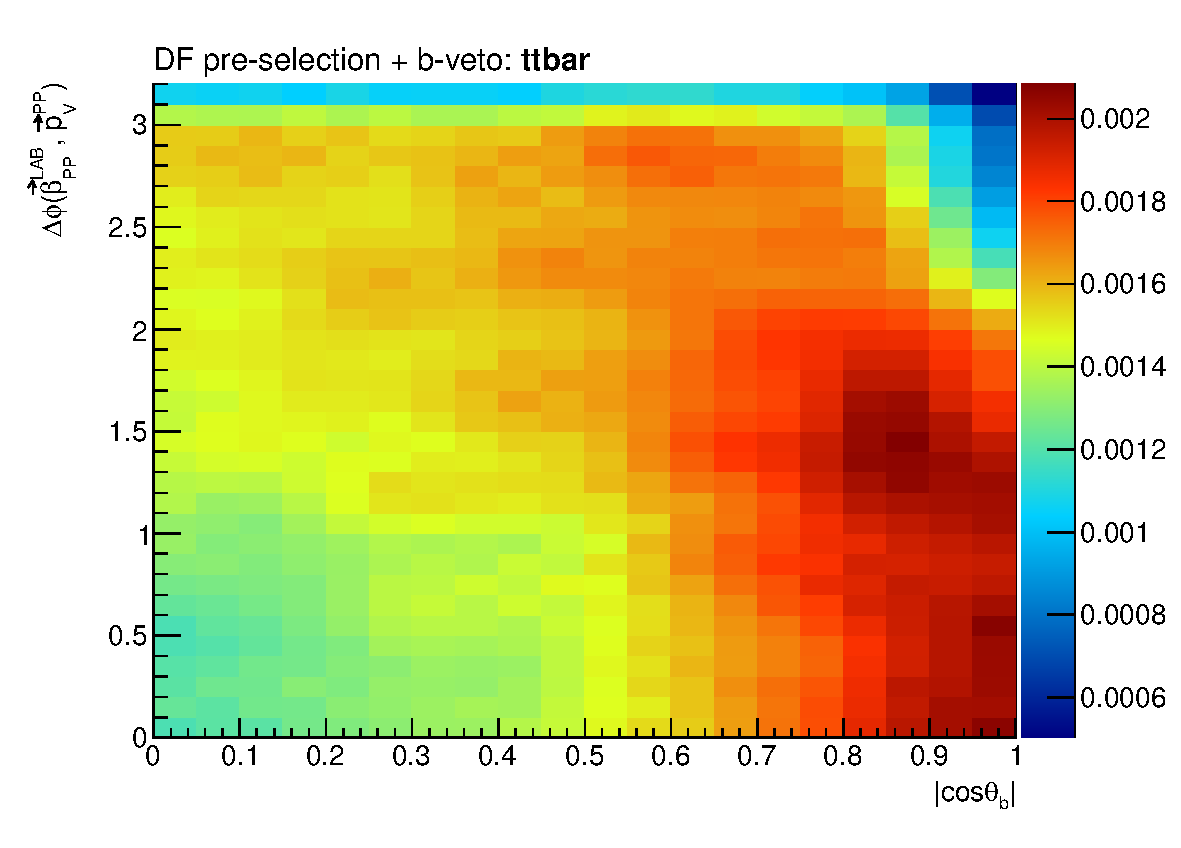
\includegraphics[width=0.48\textwidth]{figures/search_stop2l/strategy/corr2d/wwbveto_cosThetaB_DPB_vSS_ttbar_2d}
        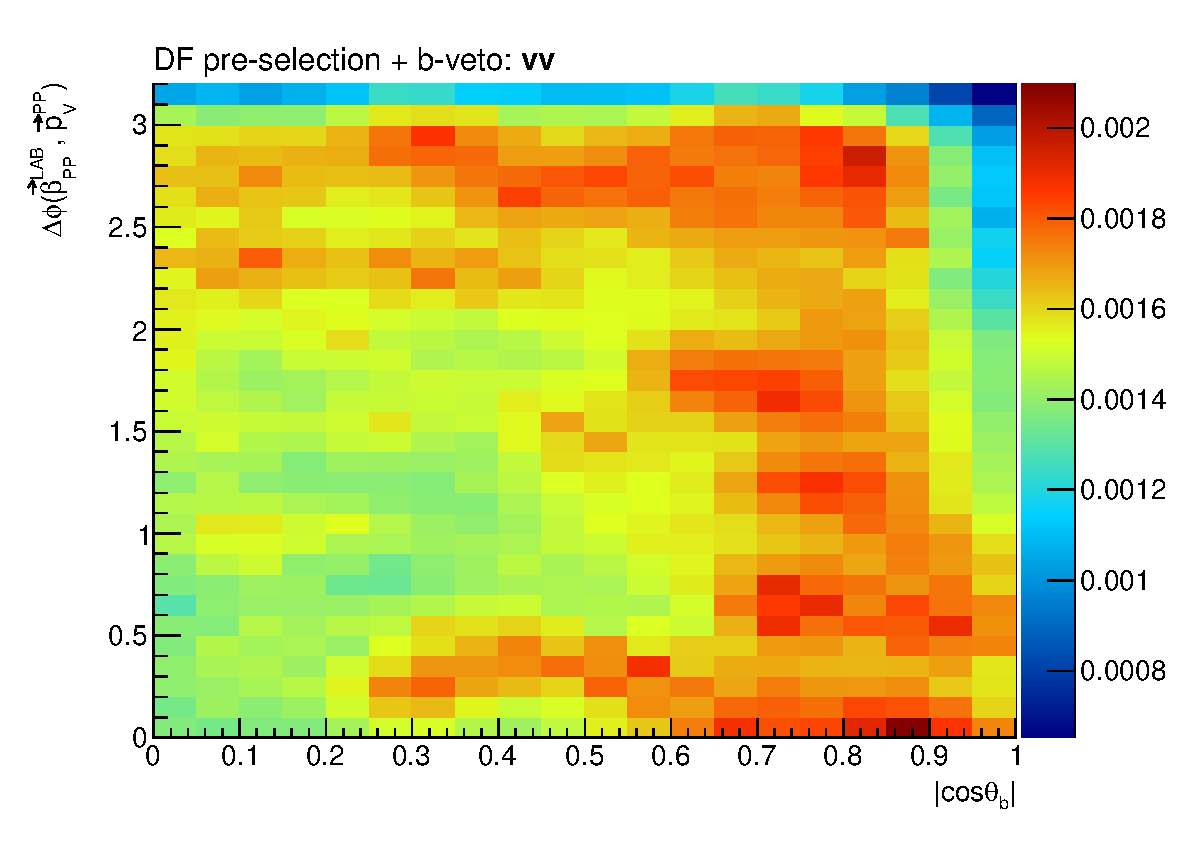
\includegraphics[width=0.48\textwidth]{figures/search_stop2l/strategy/corr2d/wwbveto_cosThetaB_DPB_vSS_vv_2d}
        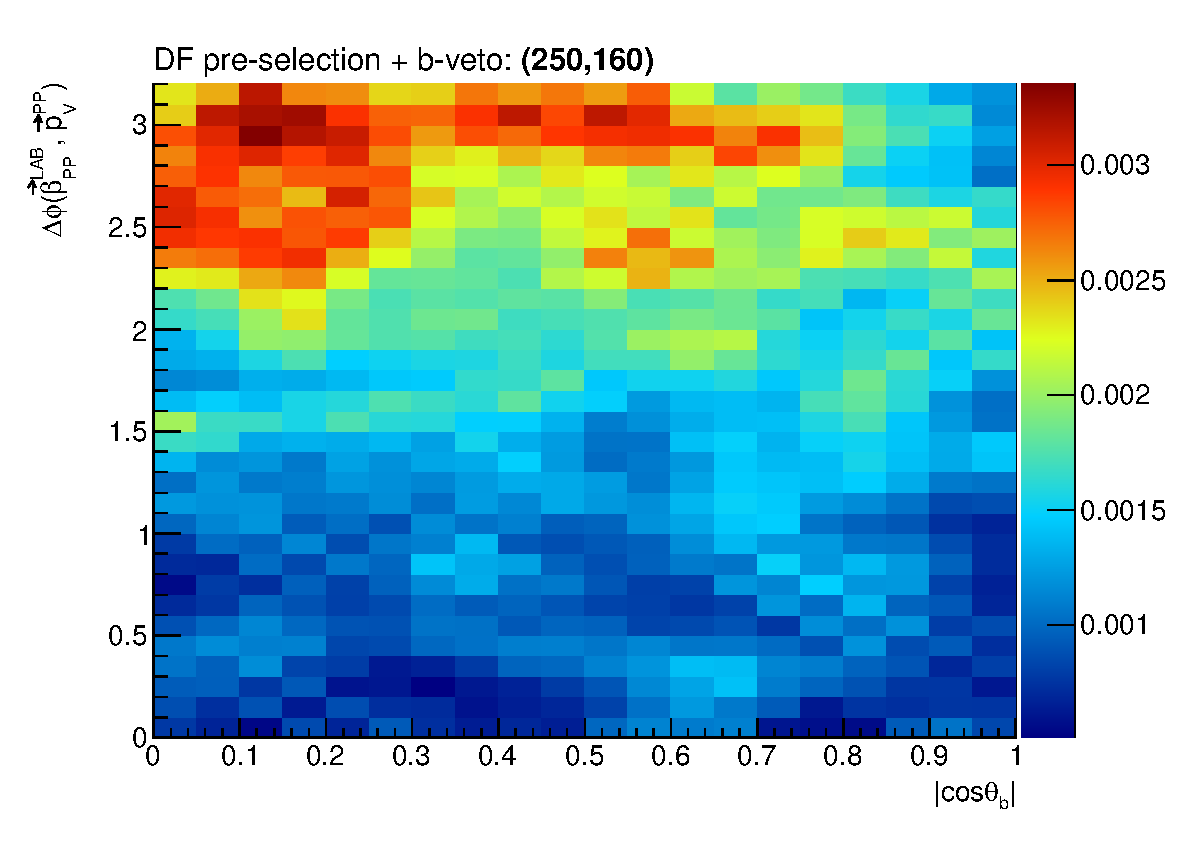
\includegraphics[width=0.48\textwidth]{figures/search_stop2l/strategy/corr2d/wwbveto_cosThetaB_DPB_vSS_bwn250_160_2d}
        \caption{
            Two-dimensional relationship between \dpb and \cosb for SM \ttbar~(\textit{upper left}),
            SM diboson processes (\textit{upper right}), and the \bWN decay with $\msn = (250, 160)$\,GeV
            (\textit{bottom}).
            The selection applied to the events populating these distributions follows the DF Preselection outlined in Table~\ref{tab:stop_preselection}
            with the additional requirement that there be no $b$-tagged jets in the event.
            The distributions are normalized, so only the shapes are relevant for comparison.
        }
        \label{fig:stop_corr2d_bveto}
    \end{center}
\end{figure}

\begin{figure}[!htb]
    \begin{center}
        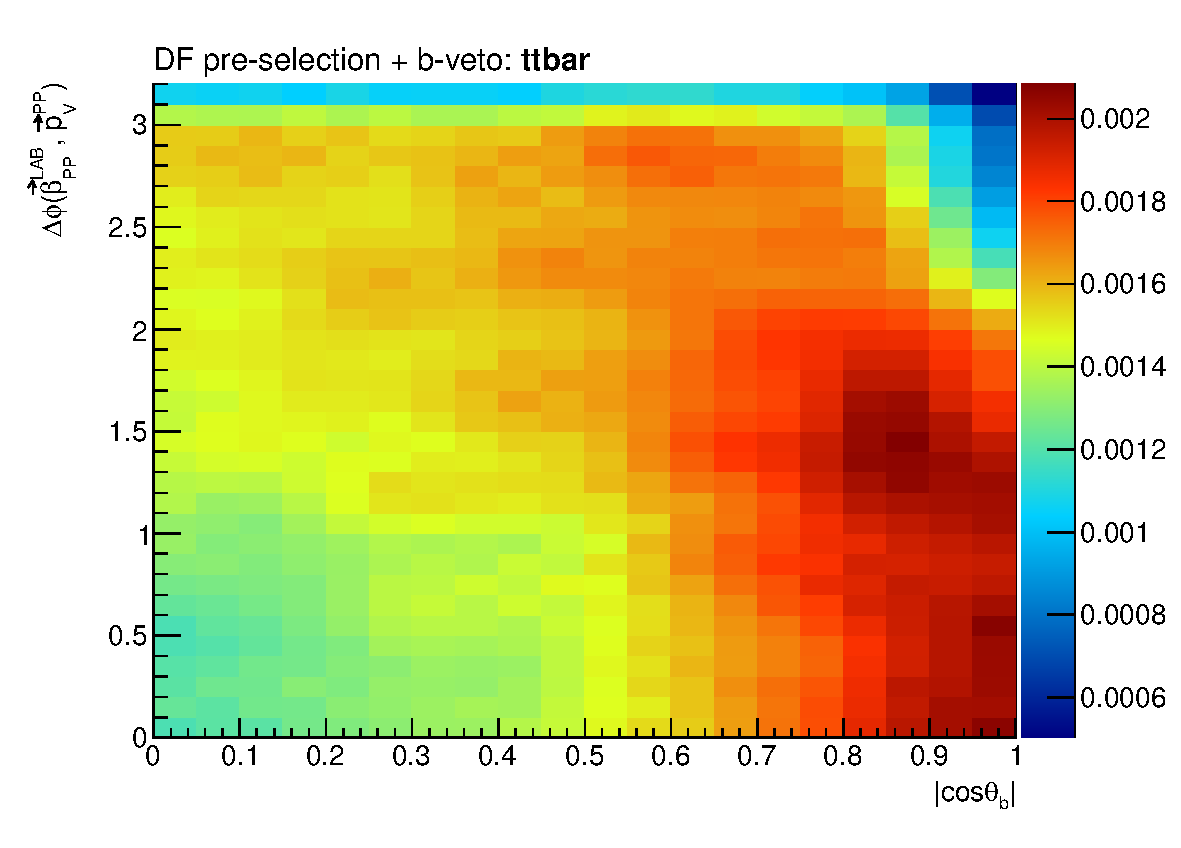
\includegraphics[width=0.48\textwidth]{figures/search_stop2l/strategy/corr2d/wwbveto_cosThetaB_DPB_vSS_ttbar_2d}
        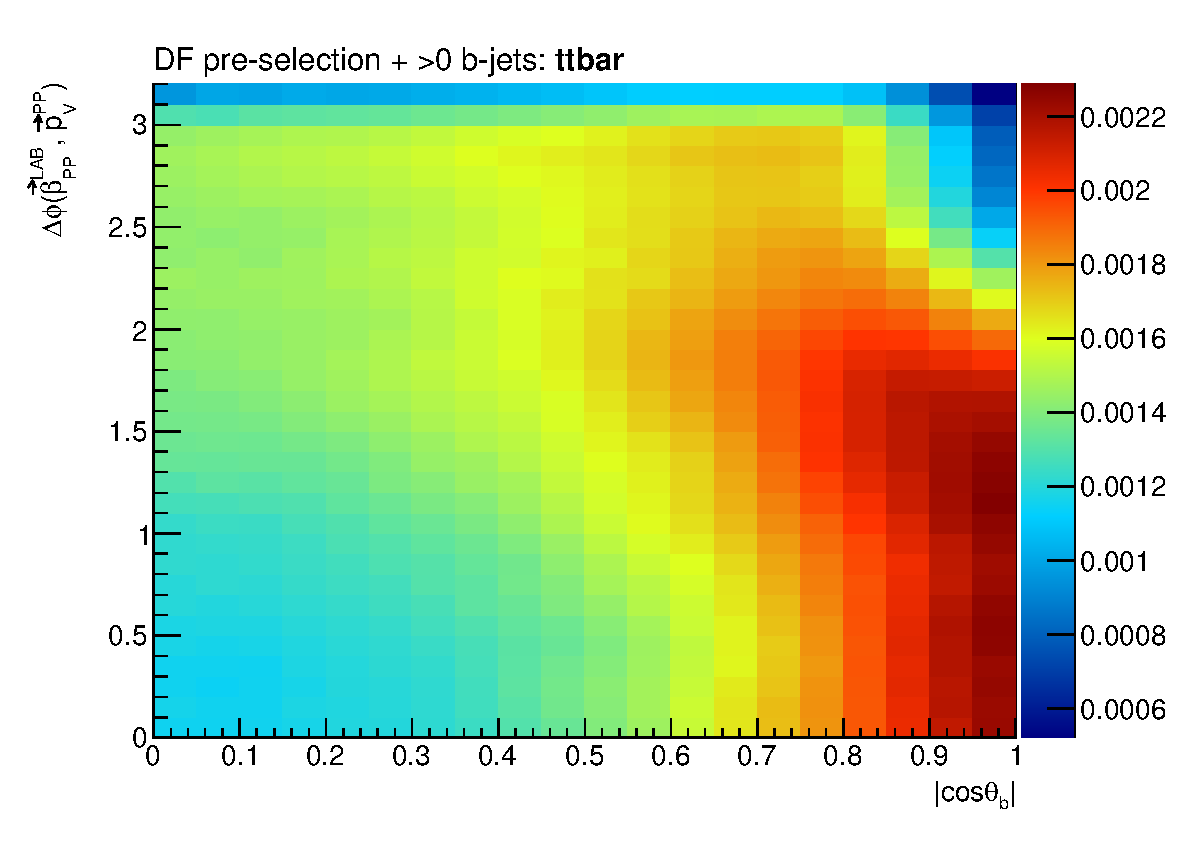
\includegraphics[width=0.48\textwidth]{figures/search_stop2l/strategy/corr2d/wwb_cosThetaB_DPB_vSS_ttbar_2d}
        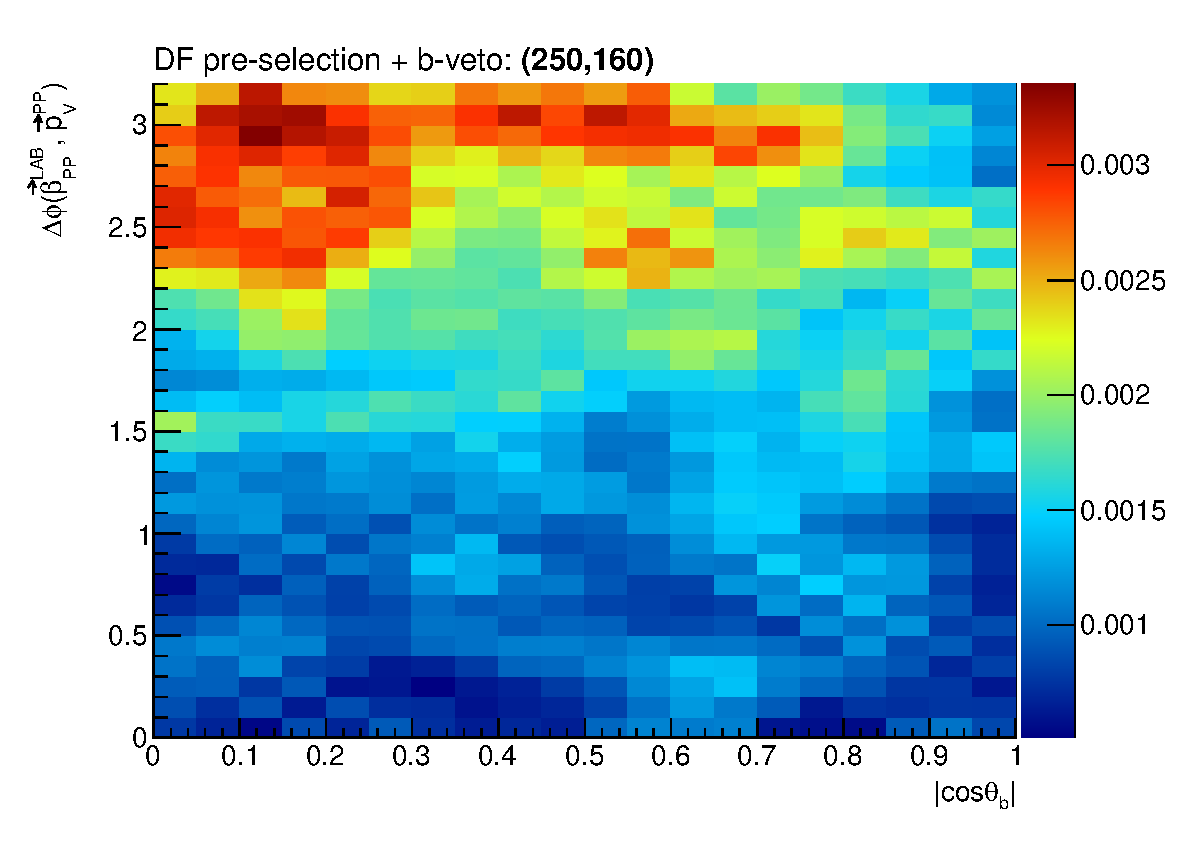
\includegraphics[width=0.48\textwidth]{figures/search_stop2l/strategy/corr2d/wwbveto_cosThetaB_DPB_vSS_bwn250_160_2d}
        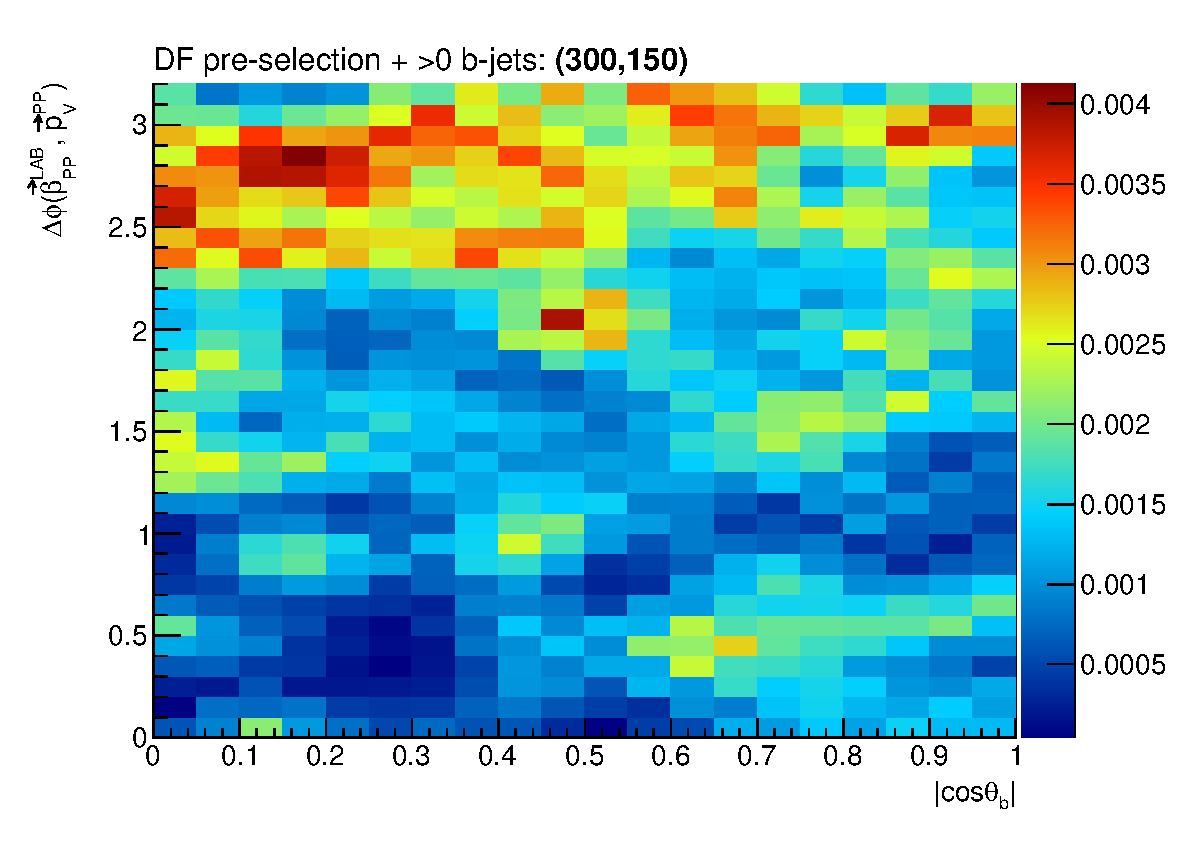
\includegraphics[width=0.48\textwidth]{figures/search_stop2l/strategy/corr2d/wwb_cosThetaB_DPB_vSS_bwn300_150_2d}
        \caption{
            Two-dimensional relationship between \dpb and \cosb for SM \ttbar~(\textit{upper}),
            the \bWN decay with $\msn = (250, 160)$\,GeV (\textit{lower left}),
            and the \bWN decay with $\msn = (350, 150)$\,GeV (\textit{lower right}).
            The selection applied to the events populating these distributions are
            required to satisfy the DF Preselection outlined in Table~\ref{tab:stop_preselection},
            with those on the left having an additional requirement that there be no $b$-tagged
            jets in the events and those on the right requiring that there be at least one $b$-tagged
            jet in the event.
            The distributions are normalized, so only the shapes are relevant for comparison.
        }
        \label{fig:stop_corr2d_b}
    \end{center}
\end{figure}

With the above discussion in mind, the complete basis of observables used to define the SRs are given by
the following,
\begin{table}[!htb]
    \begin{center}
        \caption{
            Basis of kinematic observables for the definition of analysis regions
            in the \bWN search.
        }
        \label{tab:stop_basis}
        \begin{tabular}{c}
            \hline
            \hline
                \rpt \\
                \gaminv \\
                \cosb \\
                \dpb \\
                \mdr \\
                $b$-tagged jet multiplicity \\
            \hline
            \hline
        \end{tabular}
    \end{center}
\end{table}

\FloatBarrier
\subsubsection{Optimization Procedure}
\label{sec:stop_opt}

In order to choose the precise selection thresholds on the quantities listed in Table~\ref{tab:stop_basis},
an optimization procedure is followed.
The procedure used in the search for the \bWN decay is a brute force method, and is as follows.
A multi-dimensional scan is performed over the subset of those quantities in listed in Table~\ref{tab:stop_basis},
which are listed in Table~\ref{tab:stop_opt_scan_vars}.
The scan is done using objects (leptons and jets) that satisfy the signal level criteria,
detailed in Tables~\ref{tab:stop_lepton_def} and \ref{tab:stop_jet_def}.

\begin{table}[!htb]
    \begin{center}
        \caption{
            Kinematic observables used in the \bWN grid search optimization procedure.
        }
        \label{tab:stop_opt_scan_vars}
        \begin{tabular}{c}
            \hline
            \hline
                \rpt \\
                \gaminv \\
                m \\
                b \\
            \hline
            \hline
        \end{tabular}
    \end{center}
\end{table}
\noindent
In Table~\ref{tab:stop_opt_scan_vars}, the quantities `m' and `b' are related to the slope and y-intercept of the line in the two-dimensional
space $(\cosb, \dpb)$, as illustrated in Figure~\ref{fig:stop_2d_opt}.
\begin{figure}[!htb]
    \begin{center}
        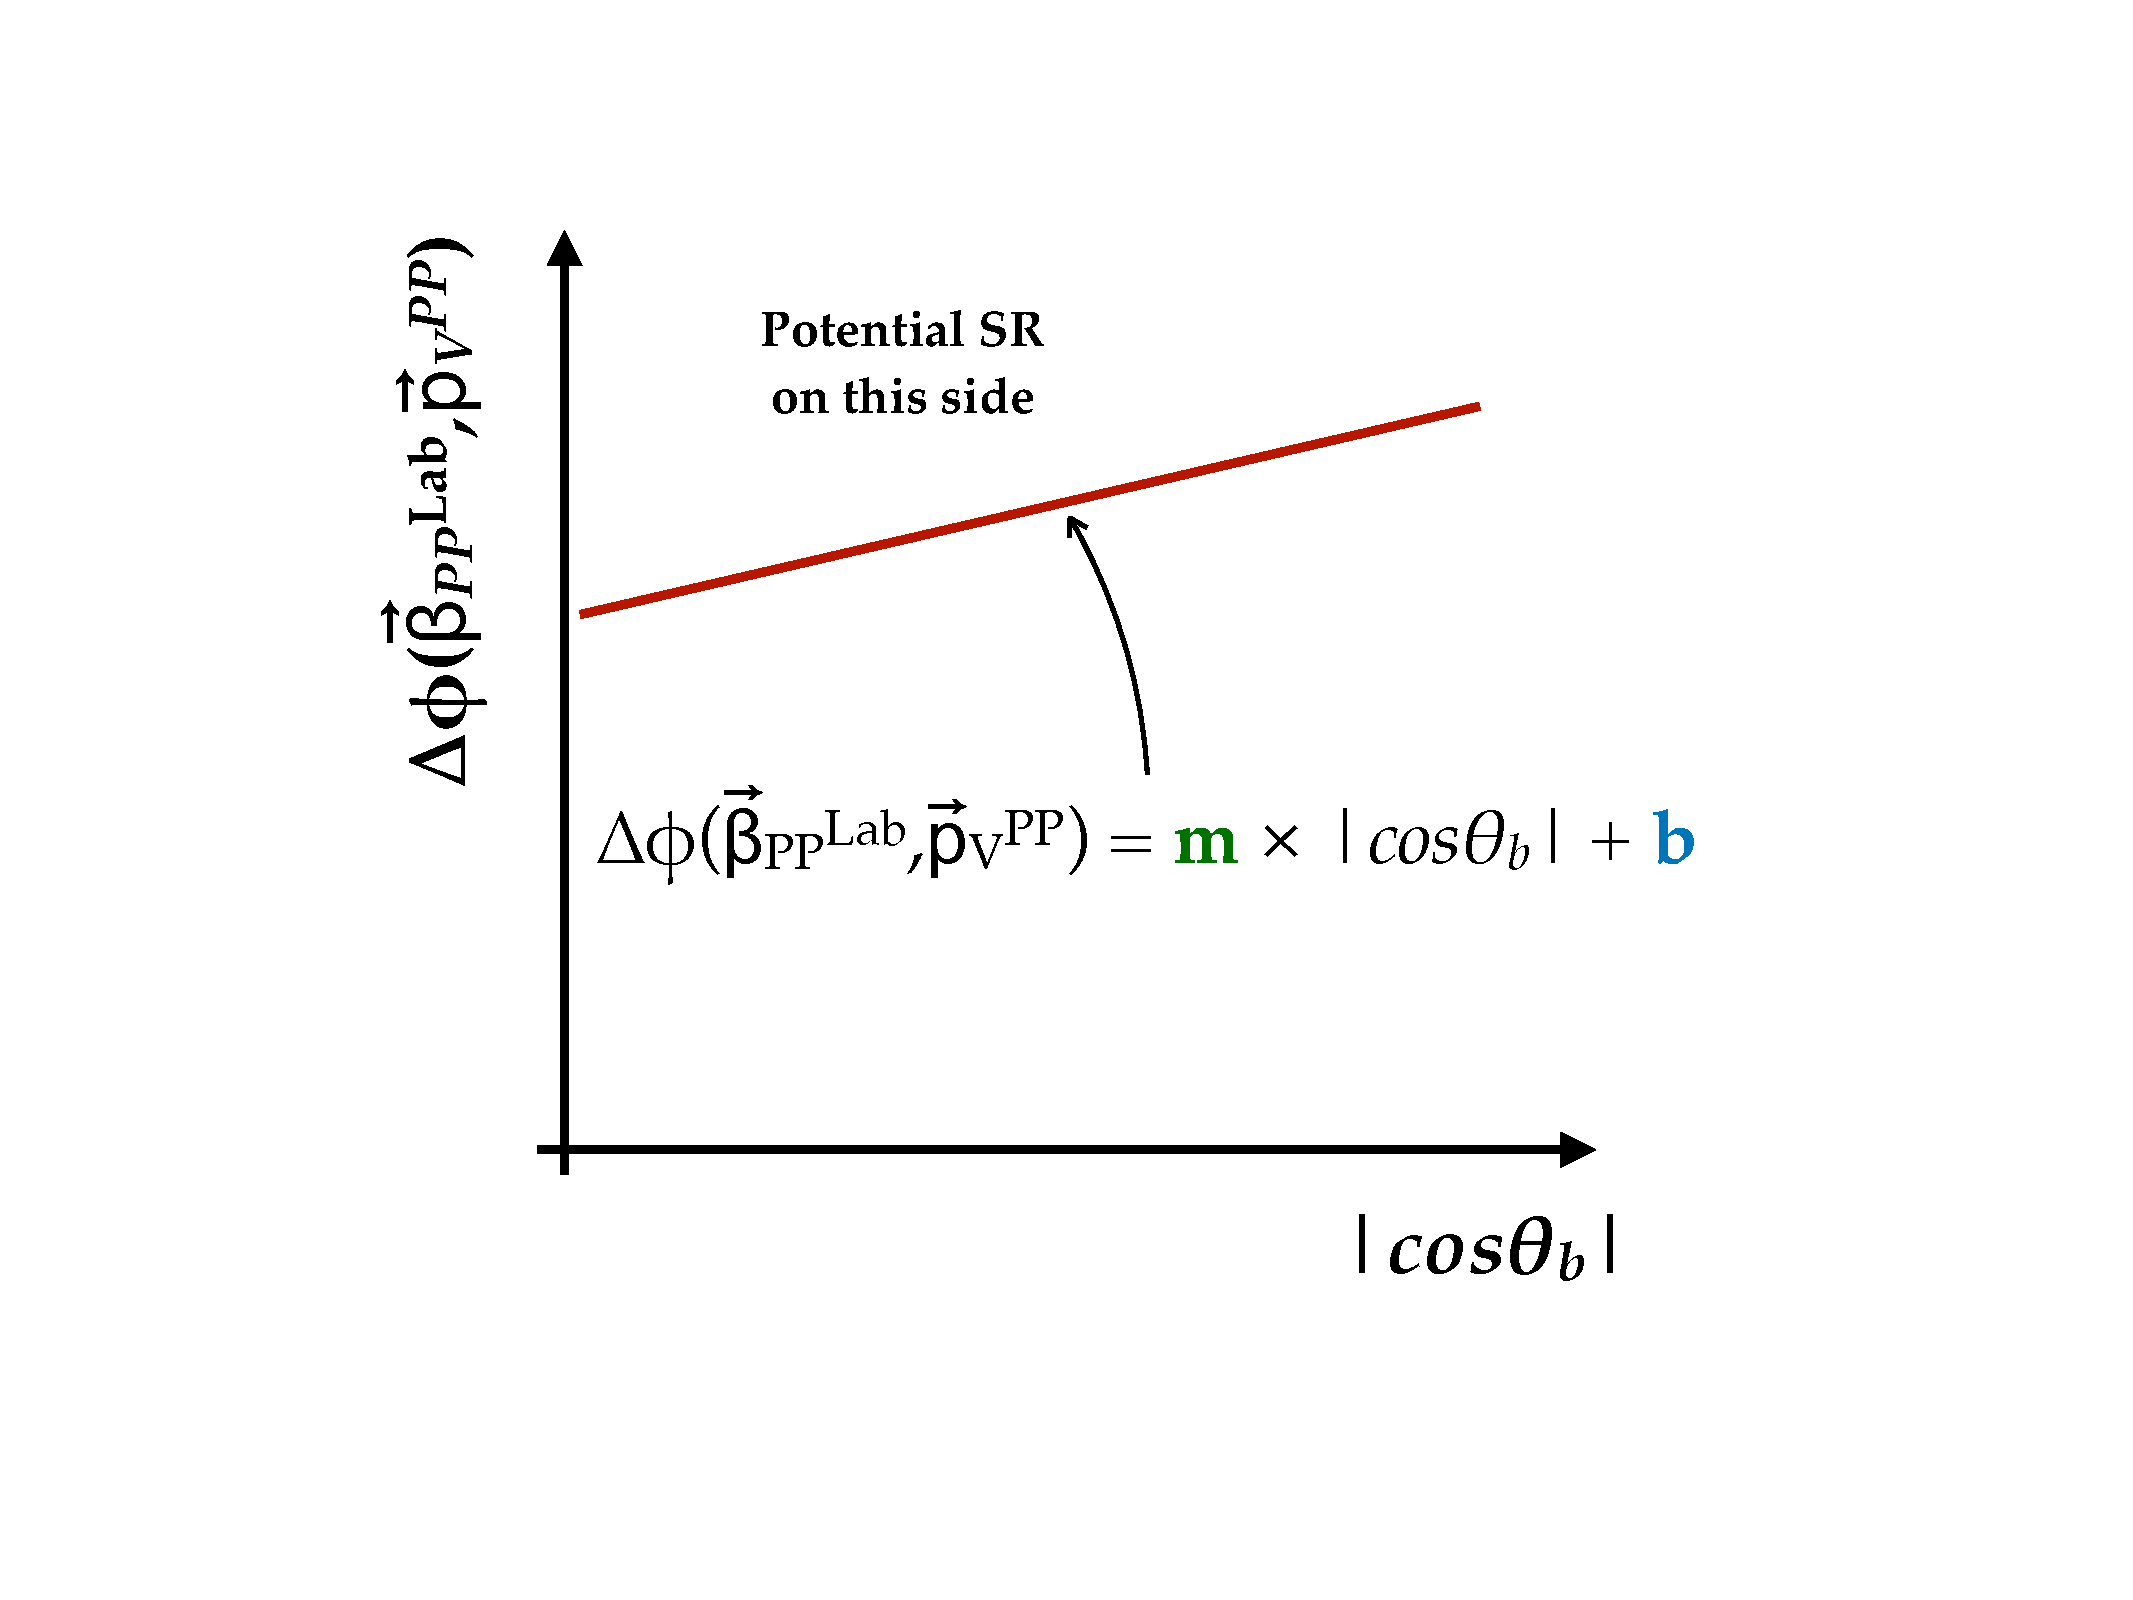
\includegraphics[width=0.5\textwidth]{figures/search_stop2l/strategy/stop_2d_optPDF}
        \caption{
        }
        \label{fig:stop_2d_opt}
    \end{center}
\end{figure}
For each of the quantites in Table~\ref{tab:stop_opt_scan_vars}, a fine-grained set of threshold
steps is defined and a multi-dimensional scan over all allowed step values for all four quantities
is performed.
At each step, a region is defined with the requirements as follows,
\begin{align*}
            \rpt &> \text{step}_{\{\rpt\}} \\
            \gaminv &> \text{step}_{\{\gaminv\}} \\
            \text{m} &= \text{step}_{\{\text{m}\}} \\
            \text{b} &= \text{step}_{\{\text{b}\}},
\end{align*}
and a metric for evaluating the sensitivity to the \bWN process of the given region
is calculated.
The metric used in the search for the \bWN process is an approximation to the Gaussian significance
associated with the discovery $p_0$-value.
The larger this quantity is, the larger the expected sensitivy to the given \bWN decay.
The significance is computed using the \textsc{RooStats} library and takes as input
the predicted number of signal events, the predicted number of background events,
and a level of uncertainty on the background event yield.\footnote{The precise
significance metric used is \href{https://root.cern.ch/doc/v606/namespaceRooStats_1_1NumberCountingUtils.html\#a4ac05df7796855dca2d8b24473bf7d4e}{RooStats::NumberCountingUtils::BinomialObsZ} 
}
Since the actual background uncertainty is unknown at the point of designing an analysis'
search regions, it is usually taken to be a conservative value.
In the the search described here, the relative background uncertainty, $\Delta b_{\text{opt}}$, was taken to be,
\begin{align*}
    \Delta b_{\text{opt}} = \sqrt{ (0.30)^2 + (\delta s)^2 },
\end{align*}
where $\delta s$ is the relative statistical uncertainty on the MC-simulated signal sample.
The quantity $\delta s$ is added in order to act as a penalty term for cases in which the
MC statistics in the signal sample become too small to give reliable estimates of the significance.

The optimisation scan is performed using only the dominant expected backgrounds, SM \ttbar~ and diboson production,
as input.
For the signal samples used to provide the estimated signal yield input,
the scan is performed three times for each of the three \textit{benchmark} signal samples with $\msn = (250, 160)$, $(300,150)$, and $(300,120)$\,GeV,
in order to assess how well each of the regions in the step procedure perform
across the three-body phase space with differing values for $\sdiff$.

At the end of the scan, there are tens of thousands of different regions checked.
The best region is chosen based on its maximization of the significance metric as well as
maintaining that there be at most 30\% statistical uncertainty on the signal and background MC samples
once the selection for the associated region is applied.
This choice is made taking into account the three benchmark \bWN signal scenarios, with the hope
of obtaining a continuous sensitivity throughout the three-body regime for scenarios
with different values of $\sdiff$.

\begin{table}[!htb]
    \begin{center}
        \caption{
            Final values obtained after performing the brute-force scan
            over the parameters listed in Table~\ref{tab:stop_opt_scan_vars}.
        }
        \label{tab:stop_scan_results}
        \begin{tabular}{l | c}
            \hline
            \hline
                \textbf{Quantity} & \textbf{Final Value Obtained from Scan} \\
                \hline
                \rpt & $0.7$ \\
                \gaminv & $0.7$ \\
                m   & $0.9$ \\
                b   & $1.6$ \\
            \hline
            \hline
        \end{tabular}
    \end{center}
\end{table}

%%%%%%%%%%%%%%%%%%%%%%%%%%%%%%%%%%%%%%%%%%%%%%%%%%%%%%%%%%%%%%%%%%%%%%%%%%%
%%%%%%%%%%%%%%%%%%%%%%%%%%%%%%%%%%%%%%%%%%%%%%%%%%%%%%%%%%%%%%%%%%%%%%%%%%%
%%%%%%%%%%%%%%%%%%%%%%%%%%%%%%%%%%%%%%%%%%%%%%%%%%%%%%%%%%%%%%%%%%%%%%%%%%%
%
% SR DEF
%
%%%%%%%%%%%%%%%%%%%%%%%%%%%%%%%%%%%%%%%%%%%%%%%%%%%%%%%%%%%%%%%%%%%%%%%%%%%
%%%%%%%%%%%%%%%%%%%%%%%%%%%%%%%%%%%%%%%%%%%%%%%%%%%%%%%%%%%%%%%%%%%%%%%%%%%
%%%%%%%%%%%%%%%%%%%%%%%%%%%%%%%%%%%%%%%%%%%%%%%%%%%%%%%%%%%%%%%%%%%%%%%%%%%
\subsubsection{Final Signal Region Definitions}

On top of the selections defined as a result of the brute-force scan, listed in Table~\ref{tab:stop_scan_results},
an \mdr requirement is added.
As the kinematic endpoint of the \mdr variable is sensitive to the (squared) mass differences
between the \stopone and \ninoone (c.f. Equation~\ref{eq:mdr_endpoint}), it is expected that the specific cut value on this
quantity will be lower for the \bWN decay scenarios with lower values of \sdiff.
The specific values of \mdr are determined by running a similar optimisation scan as detailed
in the previous section, but with only the \mdr quantity being scanned over
and with all other cuts fixed to those detailed in Table~\ref{tab:stop_scan_results}.
This is done twice, once for the benchmark signal point with $\msn = (250,160)$\,GeV and
a second time with $\msn = (350,120)$\,GeV.
The former (latter) defines the \mdr cut used for the SR targetting the \bWN decay scenarios with
$\sdiff$ nearer to $m_W$ ($m_{\text{top}}$).

The final SR definitions used in for the search for the three-body decay of the \stopone
are detailed in Table~\ref{tab:stop_sr_def}.
There are four SRs defined in total, two of which target the $\sdiff~\rightarrow~m_W$ region
and two target the $\sdiff~=~m_{\text{top}}$ region.
The former are defined by a $b$-tagged jet veto, and the latter are inclusive of
events with $b$-tagged jets.
Within each of these two categories, the SRs are further broken down by the dilepton flavor:
whether the two leptons in the events have the same-flavor (SF) or different-flavor (DF).
In order to reduce backgrounds in which the two leptons arise from the decays of $Z$-bosons,
a $Z$-veto is applied to the SF SRs by requiring that the dilepton invariant mass be outside
a 20\,\GeV window centered on the $Z$-boson mass.

The total expected background yield and composotion in terms of specific SM processes
is given in Table~\ref{tab:stop_tab_exp_sr_yield} for each of the SRs defined in Table~\ref{tab:stop_sr_def}.
It can be seen, as assumed in the text so far, that SM \ttbar~and diboson production processes
are expected to be the main SM processes contaminating the SRs.

\begin{table}[!htb]
    \begin{center}
        \caption{
            Final signal region definitions for the \bWN search.
            Selections are made after the pre-selection requirements defined in Table~\ref{tab:stop_preselection}.
            The quantities `m' and `b' are illustrated in Figure~\ref{fig:stop_2d_opt} and refer to the two-dimensional selection:
                $\dpb > m \times |\cosb| + b$.
            The lepton \pT~requirements are chosen so as to be on the dilepton trigger efficiency
            plateau.
        }
        \label{tab:stop_sr_def}
        \begin{tabular}{l | c  c  c  c}
            \hline
            \hline
            \multicolumn{5}{c}{\textbf{Signal Region Definitions for the \bWN Search}} \\
            \hline
                    & \multicolumn{4}{c}{\textbf{Common Selection}} \\
            \hline
            Lead lepton \pT [GeV] & \multicolumn{4}{c}{$>25$} \\
            Sub-lead lepton \pT [GeV] & \multicolumn{4}{c}{$>20$} \\
            \rpt    & \multicolumn{4}{c}{$>0.7$} \\
            \gaminv & \multicolumn{4}{c}{$>0.7$} \\
            m   & \multicolumn{4}{c}{$0.9$} \\
            b   & \multicolumn{4}{c}{$1.6$} \\
            \hline
                & \multicolumn{1}{c|}{\textbf{SRw-SF}} & \multicolumn{1}{c|}{\textbf{SRw-DF}} & \multicolumn{1}{c|}{\textbf{SRt-SF}} & \textbf{SRt-DF} \\
            \hline
            Dilepton invariant mass, $m_{\ell\ell}$ [GeV] & $|m_{\ell\ell} - 91.2| > 20$ & \multicolumn{1}{c|}{no req.} & $|m_{\ell\ell} - 91.2| > 20$ & no req. \\
            $b$-tagged jet multiplicity & \multicolumn{2}{c|}{Exactly 0} & \multicolumn{2}{c}{$>0$} \\
            \mdr    & \multicolumn{2}{c|}{$>95$} & \multicolumn{2}{c}{$>110$} \\
            \hline
            \hline
        \end{tabular}
    \end{center}
\end{table}

\begin{table}[!htb]
    \begin{center}
        \caption{
            Expected SM background processes in the SRs for the \bWN search,
            defined in Table~\ref{tab:stop_sr_def}.
            The bottom two rows show the predicted yields for two of the
            \bWN benchmark scenarios.
            The errors on the quoted yields are due to statistical and
            systematic uncertainties.
        }
        \label{tab:stop_tab_exp_sr_yield}
        \begin{tabular}{l | c c c c}
            \hline
            \hline
                \textbf{Process}    & \textbf{SRw-SF} & \textbf{SRw-DF} & \textbf{SRt-SF} & \textbf{SRt-DF} \\
            \hline
            Total Expected SM & $10.94 \pm 3.60$ & $8.74 \pm 3.45$ & $3.00 \pm 1.59$ & $4.62 \pm 2.38$ \\
            \hline
            \ttbar  & $4.32 \pm 2.42$ & $4.73 \pm 2.82$         & $2.41 \pm 1.54$ & $3.38 \pm 2.31$ \\
            Single-top & $0.31 \pm 0.19$ & $0.23 \pm 0.07$      & $0.12 \pm 0.015$ & $0.15 \pm 0.09$  \\
            Diboson & $3.76 \pm 1.71$ & $3.03 \pm 1.33$         & $0.16 \pm 0.05$ & $0.00 \pm 0.00$ \\
            $Z$+jets & $1.52 \pm 0.79$ & $0.05 \pm 0.01$        & $0.10 \pm 0.03$ & $0.00 \pm 0.00$  \\
            $\ttbar+V$ & $0.04 \pm 0.01$ & $0.11\pm 0.03$       & $0.21 \pm 0.06$ & $0.24 \pm 0.09$ \\
            Fakes & $0.99 \pm 0.52$ & $0.59 \pm 0.29$           & $0.00 \pm 0.00$ & $0.82 \pm 0.23$ \\
            \hline
            \bWN, $\msn = (250,160)$\,GeV & $15.06 \pm 1.78$ & $18.93 \pm 1.86$ & $3.34 \pm 0.84$ & $4.06 \pm 0.97$ \\
            \bWN, $\msn = (300,150)$\,GeV & $4.47\pm1.09$ & $7.03 \pm 1.45$ & $11.43 \pm 2.00$ & $12.86 \pm 1.97$  \\
            \hline
            \hline
        \end{tabular}
    \end{center}
\end{table}

